% Options for packages loaded elsewhere
%DIF LATEXDIFF DIFFERENCE FILE
%DIF DEL LMAms_main_old.tex   Tue Jan 28 08:16:20 2025
%DIF ADD LMAms_main.tex       Tue Jan 28 08:16:01 2025
\PassOptionsToPackage{unicode}{hyperref}
\PassOptionsToPackage{hyphens}{url}
\PassOptionsToPackage{dvipsnames,svgnames,x11names}{xcolor}
%
\documentclass[
  12pt,
  letterpaper,
  DIV=11,
  numbers=noendperiod]{scrartcl}

\usepackage{amsmath,amssymb}
\usepackage{iftex}
\ifPDFTeX
  \usepackage[T1]{fontenc}
  \usepackage[utf8]{inputenc}
  \usepackage{textcomp} % provide euro and other symbols
\else % if luatex or xetex
  \usepackage{unicode-math}
  \defaultfontfeatures{Scale=MatchLowercase}
  \defaultfontfeatures[\rmfamily]{Ligatures=TeX,Scale=1}
\fi
\usepackage{lmodern}
\ifPDFTeX\else  
    % xetex/luatex font selection
\fi
% Use upquote if available, for straight quotes in verbatim environments
\IfFileExists{upquote.sty}{\usepackage{upquote}}{}
\IfFileExists{microtype.sty}{% use microtype if available
  \usepackage[]{microtype}
  \UseMicrotypeSet[protrusion]{basicmath} % disable protrusion for tt fonts
}{}
\makeatletter
\@ifundefined{KOMAClassName}{% if non-KOMA class
  \IfFileExists{parskip.sty}{%
    \usepackage{parskip}
  }{% else
    \setlength{\parindent}{0pt}
    \setlength{\parskip}{6pt plus 2pt minus 1pt}}
}{% if KOMA class
  \KOMAoptions{parskip=half}}
\makeatother
\usepackage{xcolor}
\usepackage[margin=1in]{geometry}
\setlength{\emergencystretch}{3em} % prevent overfull lines
\setcounter{secnumdepth}{-\maxdimen} % remove section numbering
% Make \paragraph and \subparagraph free-standing
\makeatletter
\ifx\paragraph\undefined\else
  \let\oldparagraph\paragraph
  \renewcommand{\paragraph}{
    \@ifstar
      \xxxParagraphStar
      \xxxParagraphNoStar
  }
  \newcommand{\xxxParagraphStar}[1]{\oldparagraph*{#1}\mbox{}}
  \newcommand{\xxxParagraphNoStar}[1]{\oldparagraph{#1}\mbox{}}
\fi
\ifx\subparagraph\undefined\else
  \let\oldsubparagraph\subparagraph
  \renewcommand{\subparagraph}{
    \@ifstar
      \xxxSubParagraphStar
      \xxxSubParagraphNoStar
  }
  \newcommand{\xxxSubParagraphStar}[1]{\oldsubparagraph*{#1}\mbox{}}
  \newcommand{\xxxSubParagraphNoStar}[1]{\oldsubparagraph{#1}\mbox{}}
\fi
\makeatother


\providecommand{\tightlist}{%
  \setlength{\itemsep}{0pt}\setlength{\parskip}{0pt}}\usepackage{longtable,booktabs,array}
\usepackage{calc} % for calculating minipage widths
% Correct order of tables after \paragraph or \subparagraph
\usepackage{etoolbox}
\makeatletter
\patchcmd\longtable{\par}{\if@noskipsec\mbox{}\fi\par}{}{}
\makeatother
% Allow footnotes in longtable head/foot
\IfFileExists{footnotehyper.sty}{\usepackage{footnotehyper}}{\usepackage{footnote}}
\makesavenoteenv{longtable}
\usepackage{graphicx}
\makeatletter
\def\maxwidth{\ifdim\Gin@nat@width>\linewidth\linewidth\else\Gin@nat@width\fi}
\def\maxheight{\ifdim\Gin@nat@height>\textheight\textheight\else\Gin@nat@height\fi}
\makeatother
% Scale images if necessary, so that they will not overflow the page
% margins by default, and it is still possible to overwrite the defaults
% using explicit options in \includegraphics[width, height, ...]{}
\setkeys{Gin}{width=\maxwidth,height=\maxheight,keepaspectratio}
% Set default figure placement to htbp
\makeatletter
\def\fps@figure{htbp}
\makeatother
% definitions for citeproc citations
\NewDocumentCommand\citeproctext{}{}
\NewDocumentCommand\citeproc{mm}{%
  \begingroup\def\citeproctext{#2}\cite{#1}\endgroup}
\makeatletter
 % allow citations to break across lines
 \let\@cite@ofmt\@firstofone
 % avoid brackets around text for \cite:
 \def\@biblabel#1{}
 \def\@cite#1#2{{#1\if@tempswa , #2\fi}}
\makeatother
\newlength{\cslhangindent}
\setlength{\cslhangindent}{1.5em}
\newlength{\csllabelwidth}
\setlength{\csllabelwidth}{3em}
\newenvironment{CSLReferences}[2] % #1 hanging-indent, #2 entry-spacing
 {\begin{list}{}{%
  \setlength{\itemindent}{0pt}
  \setlength{\leftmargin}{0pt}
  \setlength{\parsep}{0pt}
  % turn on hanging indent if param 1 is 1
  \ifodd #1
   \setlength{\leftmargin}{\cslhangindent}
   \setlength{\itemindent}{-1\cslhangindent}
  \fi
  % set entry spacing
  \setlength{\itemsep}{#2\baselineskip}}}
 {\end{list}}
\usepackage{calc}
\newcommand{\CSLBlock}[1]{\hfill\break\parbox[t]{\linewidth}{\strut\ignorespaces#1\strut}}
\newcommand{\CSLLeftMargin}[1]{\parbox[t]{\csllabelwidth}{\strut#1\strut}}
\newcommand{\CSLRightInline}[1]{\parbox[t]{\linewidth - \csllabelwidth}{\strut#1\strut}}
\newcommand{\CSLIndent}[1]{\hspace{\cslhangindent}#1}

\usepackage{booktabs}
\usepackage{longtable}
\usepackage{array}
\usepackage{multirow}
\usepackage{wrapfig}
\usepackage{float}
\usepackage{colortbl}
\usepackage{pdflscape}
\usepackage{tabu}
\usepackage{threeparttable}
\usepackage{threeparttablex}
\usepackage[normalem]{ulem}
\usepackage{makecell}
\usepackage{xcolor}
\usepackage[default]{sourcesanspro}
\usepackage{sourcecodepro}
\usepackage{lineno}
\linenumbers
\linespread{1.2}
\KOMAoption{captions}{tableheading}
\makeatletter
\@ifpackageloaded{caption}{}{\usepackage{caption}}
\AtBeginDocument{%
\ifdefined\contentsname
  \renewcommand*\contentsname{Table of contents}
\else
  \newcommand\contentsname{Table of contents}
\fi
\ifdefined\listfigurename
  \renewcommand*\listfigurename{List of Figures}
\else
  \newcommand\listfigurename{List of Figures}
\fi
\ifdefined\listtablename
  \renewcommand*\listtablename{List of Tables}
\else
  \newcommand\listtablename{List of Tables}
\fi
\ifdefined\figurename
  \renewcommand*\figurename{Fig.}
\else
  \newcommand\figurename{Fig.}
\fi
\ifdefined\tablename
  \renewcommand*\tablename{Table}
\else
  \newcommand\tablename{Table}
\fi
}
\@ifpackageloaded{float}{}{\usepackage{float}}
\floatstyle{ruled}
\@ifundefined{c@chapter}{\newfloat{codelisting}{h}{lop}}{\newfloat{codelisting}{h}{lop}[chapter]}
\floatname{codelisting}{Listing}
\newcommand*\listoflistings{\listof{codelisting}{List of Listings}}
\makeatother
\makeatletter
\makeatother
\makeatletter
\@ifpackageloaded{caption}{}{\usepackage{caption}}
\@ifpackageloaded{subcaption}{}{\usepackage{subcaption}}
\makeatother

\ifLuaTeX
  \usepackage{selnolig}  % disable illegal ligatures
\fi
\usepackage{bookmark}

\IfFileExists{xurl.sty}{\usepackage{xurl}}{} % add URL line breaks if available
\urlstyle{same} % disable monospaced font for URLs
\hypersetup{
  colorlinks=true,
  linkcolor={blue},
  filecolor={Maroon},
  citecolor={Blue},
  urlcolor={Blue},
  pdfcreator={LaTeX via pandoc}}


\author{}
\date{}
%DIF PREAMBLE EXTENSION ADDED BY LATEXDIFF
%DIF UNDERLINE PREAMBLE %DIF PREAMBLE
\RequirePackage[normalem]{ulem} %DIF PREAMBLE
\RequirePackage{color}\definecolor{RED}{rgb}{1,0,0}\definecolor{BLUE}{rgb}{0,0,1} %DIF PREAMBLE
\providecommand{\DIFadd}[1]{{\protect\color{blue}\uwave{#1}}} %DIF PREAMBLE
\providecommand{\DIFdel}[1]{{\protect\color{red}\sout{#1}}}                      %DIF PREAMBLE
%DIF SAFE PREAMBLE %DIF PREAMBLE
\providecommand{\DIFaddbegin}{} %DIF PREAMBLE
\providecommand{\DIFaddend}{} %DIF PREAMBLE
\providecommand{\DIFdelbegin}{} %DIF PREAMBLE
\providecommand{\DIFdelend}{} %DIF PREAMBLE
\providecommand{\DIFmodbegin}{} %DIF PREAMBLE
\providecommand{\DIFmodend}{} %DIF PREAMBLE
%DIF FLOATSAFE PREAMBLE %DIF PREAMBLE
\providecommand{\DIFaddFL}[1]{\DIFadd{#1}} %DIF PREAMBLE
\providecommand{\DIFdelFL}[1]{\DIFdel{#1}} %DIF PREAMBLE
\providecommand{\DIFaddbeginFL}{} %DIF PREAMBLE
\providecommand{\DIFaddendFL}{} %DIF PREAMBLE
\providecommand{\DIFdelbeginFL}{} %DIF PREAMBLE
\providecommand{\DIFdelendFL}{} %DIF PREAMBLE
\newcommand{\DIFscaledelfig}{0.5}
%DIF HIGHLIGHTGRAPHICS PREAMBLE %DIF PREAMBLE
\RequirePackage{settobox} %DIF PREAMBLE
\RequirePackage{letltxmacro} %DIF PREAMBLE
\newsavebox{\DIFdelgraphicsbox} %DIF PREAMBLE
\newlength{\DIFdelgraphicswidth} %DIF PREAMBLE
\newlength{\DIFdelgraphicsheight} %DIF PREAMBLE
% store original definition of \includegraphics %DIF PREAMBLE
\LetLtxMacro{\DIFOincludegraphics}{\includegraphics} %DIF PREAMBLE
\newcommand{\DIFaddincludegraphics}[2][]{{\color{blue}\fbox{\DIFOincludegraphics[#1]{#2}}}} %DIF PREAMBLE
\newcommand{\DIFdelincludegraphics}[2][]{% %DIF PREAMBLE
\sbox{\DIFdelgraphicsbox}{\DIFOincludegraphics[#1]{#2}}% %DIF PREAMBLE
\settoboxwidth{\DIFdelgraphicswidth}{\DIFdelgraphicsbox} %DIF PREAMBLE
\settoboxtotalheight{\DIFdelgraphicsheight}{\DIFdelgraphicsbox} %DIF PREAMBLE
\scalebox{\DIFscaledelfig}{% %DIF PREAMBLE
\parbox[b]{\DIFdelgraphicswidth}{\usebox{\DIFdelgraphicsbox}\\[-\baselineskip] \rule{\DIFdelgraphicswidth}{0em}}\llap{\resizebox{\DIFdelgraphicswidth}{\DIFdelgraphicsheight}{% %DIF PREAMBLE
\setlength{\unitlength}{\DIFdelgraphicswidth}% %DIF PREAMBLE
\begin{picture}(1,1)% %DIF PREAMBLE
\thicklines\linethickness{2pt} %DIF PREAMBLE
{\color[rgb]{1,0,0}\put(0,0){\framebox(1,1){}}}% %DIF PREAMBLE
{\color[rgb]{1,0,0}\put(0,0){\line( 1,1){1}}}% %DIF PREAMBLE
{\color[rgb]{1,0,0}\put(0,1){\line(1,-1){1}}}% %DIF PREAMBLE
\end{picture}% %DIF PREAMBLE
}\hspace*{3pt}}} %DIF PREAMBLE
} %DIF PREAMBLE
\LetLtxMacro{\DIFOaddbegin}{\DIFaddbegin} %DIF PREAMBLE
\LetLtxMacro{\DIFOaddend}{\DIFaddend} %DIF PREAMBLE
\LetLtxMacro{\DIFOdelbegin}{\DIFdelbegin} %DIF PREAMBLE
\LetLtxMacro{\DIFOdelend}{\DIFdelend} %DIF PREAMBLE
\DeclareRobustCommand{\DIFaddbegin}{\DIFOaddbegin \let\includegraphics\DIFaddincludegraphics} %DIF PREAMBLE
\DeclareRobustCommand{\DIFaddend}{\DIFOaddend \let\includegraphics\DIFOincludegraphics} %DIF PREAMBLE
\DeclareRobustCommand{\DIFdelbegin}{\DIFOdelbegin \let\includegraphics\DIFdelincludegraphics} %DIF PREAMBLE
\DeclareRobustCommand{\DIFdelend}{\DIFOaddend \let\includegraphics\DIFOincludegraphics} %DIF PREAMBLE
\LetLtxMacro{\DIFOaddbeginFL}{\DIFaddbeginFL} %DIF PREAMBLE
\LetLtxMacro{\DIFOaddendFL}{\DIFaddendFL} %DIF PREAMBLE
\LetLtxMacro{\DIFOdelbeginFL}{\DIFdelbeginFL} %DIF PREAMBLE
\LetLtxMacro{\DIFOdelendFL}{\DIFdelendFL} %DIF PREAMBLE
\DeclareRobustCommand{\DIFaddbeginFL}{\DIFOaddbeginFL \let\includegraphics\DIFaddincludegraphics} %DIF PREAMBLE
\DeclareRobustCommand{\DIFaddendFL}{\DIFOaddendFL \let\includegraphics\DIFOincludegraphics} %DIF PREAMBLE
\DeclareRobustCommand{\DIFdelbeginFL}{\DIFOdelbeginFL \let\includegraphics\DIFdelincludegraphics} %DIF PREAMBLE
\DeclareRobustCommand{\DIFdelendFL}{\DIFOaddendFL \let\includegraphics\DIFOincludegraphics} %DIF PREAMBLE
%DIF LISTINGS PREAMBLE %DIF PREAMBLE
\RequirePackage{listings} %DIF PREAMBLE
\RequirePackage{color} %DIF PREAMBLE
\lstdefinelanguage{DIFcode}{ %DIF PREAMBLE
%DIF DIFCODE_UNDERLINE %DIF PREAMBLE
  moredelim=[il][\color{red}\sout]{\%DIF\ <\ }, %DIF PREAMBLE
  moredelim=[il][\color{blue}\uwave]{\%DIF\ >\ } %DIF PREAMBLE
} %DIF PREAMBLE
\lstdefinestyle{DIFverbatimstyle}{ %DIF PREAMBLE
	language=DIFcode, %DIF PREAMBLE
	basicstyle=\ttfamily, %DIF PREAMBLE
	columns=fullflexible, %DIF PREAMBLE
	keepspaces=true %DIF PREAMBLE
} %DIF PREAMBLE
\lstnewenvironment{DIFverbatim}{\lstset{style=DIFverbatimstyle}}{} %DIF PREAMBLE
\lstnewenvironment{DIFverbatim*}{\lstset{style=DIFverbatimstyle,showspaces=true}}{} %DIF PREAMBLE
%DIF END PREAMBLE EXTENSION ADDED BY LATEXDIFF

\begin{document}


\textbf{Decomposing leaf mass into metabolic and structural components
explains divergent patterns of trait variation within and among plant
species}\\
\strut \\
Masatoshi Katabuchi\textsuperscript{1,2*}, Kaoru
Kitajima\textsuperscript{2,3,4}, S. Joseph Wright\textsuperscript{4},
Sunshine A. Van Bael\textsuperscript{4,5}, Jeanne L. D.
Osnas\textsuperscript{2} and Jeremy W. Lichstein\textsuperscript{2}\\
\strut \\
\textsuperscript{1} Xishuangbanna Tropical Botanical Garden, Chinese
Academy of Sciences, Menglun, Yunnan 666303 China

\textsuperscript{2} Department of Biology, University of Florida,
Gainesville, FL 32611, USA

\textsuperscript{3} Graduate School of Agriculture, Kyoto University,
Kitashirakawa Oiwake-Cho, Kyoto 606-8502 Japan

\textsuperscript{4} Smithsonian Tropical Research Institute, 9100 Panama
City Pl., Washington, DC 20521

\textsuperscript{5} Department of Ecology and Evolutionary Biology,
Tulane University, New Orleans, LA 70118 USA

\textbf{*Corresponding Author}: E-mail:
\href{mailto:katabuchi@xtbg.ac.cn}{\nolinkurl{katabuchi@xtbg.ac.cn}};
\href{mailto:mattocci27@gmail.com}{\nolinkurl{mattocci27@gmail.com}}

Masatoshi Katabuchi: \url{https://orcid.org/0000-0001-9900-9029}

Kaoru Kitajima: \url{https://orcid.org/0000-0001-6822-8536}

Sunshine A. Van Bael: \url{https://orcid.org/0000-0001-7317-3533}

S. Joseph Wright: \url{https://orcid.org/0000-0003-4260-5676}

Jeremy W. Lichstein: \url{https://orcid.org/0000-0001-5553-6142}\\
\strut \\
\textbf{Keywords:} Bayesian inference, functional diversity, global
vegetation models, latent variables, optimal leaf lifespan

Author Contributions: MK, JWL and JLDO conceived of the study. KK
provided guidance on leaf physiology and interpreting trait data. KK,
SJW and SAVB contributed data. MK devised the analytical approach and
performed analyses. MK and JWL wrote the first draft of the manuscript,
and all authors contributed to revisions.

\textbf{Abstract}

Across the global flora, interspecific variation in photosynthetic and
metabolic rates depends more strongly on leaf area than leaf mass. In
contrast, intraspecific variation in these rates is strongly
mass-dependent. These contrasting patterns suggest that the causes of
variation in leaf mass per area (LMA) may be fundamentally different
within vs.~among species. In order to explain these contrasting
patterns, we developed a statistical modeling framework to decompose LMA
into two components -- metabolic LMAm (which determines photosynthetic
capacity and dark respiration) and structural LMAs (which determines
leaf toughness and potential leaf lifespan) -- using leaf trait data
from tropical forests in Panama and a global leaf-trait database.
Decomposing LMA into LMAm and LMAs improves predictions of leaf trait
variation (photosynthesis, respiration, and lifespan) within and among
species. We show that strong area-dependence of metabolic traits across
species can result from multiple factors, including high LMAs variance
and/or a slow increase in photosynthetic capacity with increasing LMAm.
In contrast, strong mass-dependence of metabolic traits within species
results from LMAm increasing from shady to sunny conditions. LMAm and
LMAs were nearly independent of each other in both global and Panama
datasets, suggesting the presence of at least two important dimensions
of leaf functional variation.

\section{Introduction}\label{introduction}

Leaf functional traits play an important role in ecological and
physiological tradeoffs (\citeproc{ref-Wright2004a}{Wright et al. 2004};
\citeproc{ref-Reich2014}{Reich 2014}; \citeproc{ref-Onoda2017}{Onoda et
al. 2017}) and in carbon and nutrient cycling
(\citeproc{ref-Tcherkez2017}{Tcherkez et al. 2017}; e.g.,
\citeproc{ref-Huntingford2017}{Huntingford et al. 2017}). Thus,
understanding the causes and consequences of leaf trait variation is an
important goal in ecology, plant physiology, and biogeochemistry
(\citeproc{ref-Bonan2002}{Bonan et al. 2002};
\citeproc{ref-Poorter2009}{Poorter et al. 2009}). Different leaf
assemblages exhibit markedly different patterns of trait variation. For
example, across global species, whole-leaf values of traits related to
photosynthesis and metabolism (e.g., the photosynthetic capacity,
respiration rate, or nutrient content of entire leaves) tend to increase
more strongly with leaf area than leaf mass
(\citeproc{ref-Osnas2013}{Osnas et al. 2013}), whereas the opposite
pattern (strong mass-dependence of these same traits) is observed within
species across light gradients (\citeproc{ref-Osada2001}{Osada et al.
2001}; \citeproc{ref-Niinemets2015}{Niinemets et al. 2015};
\citeproc{ref-Osnas2018}{Osnas et al. 2018}). Functional groups (e.g.,
deciduous vs.~evergreen angiosperms) also differ from each other in
terms of how variation in photosynthetic and metabolic traits depends on
leaf mass and area (\citeproc{ref-Lusk2008}{Lusk et al. 2008};
\citeproc{ref-Osnas2018}{Osnas et al. 2018}). These divergent patterns
suggest the presence of multiple drivers of trait variation.

Strong interspecific correlations among leaf mass per area (LMA), leaf
lifespan (LL), and mass-normalized leaf traits related to photosynthesis
and metabolism (hereafter, `metabolic traits') have been interpreted as
evidence for a single dominant axis of leaf functional variation
(\citeproc{ref-Wright2004a}{Wright et al. 2004}). However, the
interpretation of these strong correlations, which can result from
mass-normalization of area-dependent traits
(\citeproc{ref-Lloyd2013}{Lloyd et al. 2013};
\citeproc{ref-Osnas2013}{Osnas et al. 2013}), is controversial. On the
one hand, mass-normalization has been justified based on economic
principles alone (\citeproc{ref-Kikuzawa1991}{Kikuzawa 1991};
\citeproc{ref-Westoby2013}{Westoby et al. 2013}), because leaf mass
provides a simple index of investment that underlies the leaf economics
spectrum (LES), ranging from cheap, low-LMA leaves with a fast rate of
return per-unit investment to expensive, high-LMA leaves with a slow
rate of return (\citeproc{ref-Wright2004a}{Wright et al. 2004}). On the
other hand, because the lifetime return on investment depends on LL
(\citeproc{ref-Westoby2000}{Westoby et al. 2000};
\citeproc{ref-Falster2012}{Falster et al. 2012}), leaf economics
analyses should arguably use annualized construction costs (or mass/LL),
rather than mass \emph{per se}, as an index of leaf cost
(\citeproc{ref-Osnas2013}{Osnas et al. 2013}). In global analyses,
normalizing leaf traits by mass/LL yields similarly weak correlations as
area-normalization, because leaf area is roughly proportional to mass/LL
across global species (\citeproc{ref-Osnas2013}{Osnas et al. 2013}).

Area-dependence of metabolic traits and the inconsistent correlation
strengths obtained from different normalizers
(\citeproc{ref-Lloyd2013}{Lloyd et al. 2013};
\citeproc{ref-Osnas2013}{Osnas et al. 2013}) suggest that strong
mass-based correlations should not, by themselves, be taken as strong
evidence for a single dominant axis of leaf functional diversity. The
existence of multiple important axes of leaf functional diversity would
not invalidate mass-normalization or the LES
(\citeproc{ref-Westoby2013}{Westoby et al. 2013}). This
multi-dimensionality would, however, have important implications for our
understanding of leaf function (\citeproc{ref-Niinemets2006a}{Niinemets,
and Sack 2006}; \citeproc{ref-Onoda2017}{Onoda et al. 2017}), the role
of trait variation in community assembly (e.g.,
\citeproc{ref-Falster2017}{Falster et al. 2017};
\citeproc{ref-Lichstein2021}{Lichstein et al. 2021}), and how to
accurately represent trait variation in ecosystem models, including
dynamic global vegetation models (DGVMs; e.g., Bonan et al.~2002; Fisher
et al.~2015; Sakschewski et al.~2016).

To understand why the same data can be interpreted as either supporting
or opposing the existence of a single dominant axis of leaf trait
variation, consider the conceptual model proposed by Osnas et al.
(\citeproc{ref-Osnas2018}{2018}), in which LMA is comprised of two
additive components: metabolic LMA (LMAm) -- the mass per area of
chloroplasts and other metabolically active leaf components that
contribute directly to photosynthesis and respiration -- and structural
LMA (LMAs) -- the mass per area of structural leaf components that
contribute to toughness and durability
(\citeproc{ref-Kitajima2012}{Kitajima et al. 2012},
\citeproc{ref-Kitajima2016}{2016}; \citeproc{ref-Onoda2017}{Onoda et al.
2017}). Suppose these two LMA components are independent axes of
functional variation, so that LMAm and LMAs are uncorrelated across
species (Fig.~\ref{fig-hypo}a). These two independent axes can be
translated into either a two-dimensional trait space (if metabolic
traits are area-normalized; Fig.~\ref{fig-hypo}b) or a primarily
one-dimensional trait space (if metabolic traits are mass-normalized;
Fig.~\ref{fig-hypo}c). While Fig.~\ref{fig-hypo}b and
Fig.~\ref{fig-hypo}c are both `correct' representations of the same
data, they lead to different perceptions about the dimensionality of
leaf functional variation. If LMAm, LMAs, and/or other axes are largely
independent and have distinct functional consequences, then it would not
be possible to accurately represent functional variation with a single
axis.

The hypothetical example in Fig.~\ref{fig-hypo} shows how
mass-normalization can, in principle, make a two-dimensional trait space
appear one-dimensional, but the dimensionality of functional variation
in real leaf assemblages remains an open question. One way to better
understand the dimensionality of leaf trait variation is to compare
models with different numbers of dimensions and to ask if models with
multiple dimensions provide \DIFdelbegin \DIFdel{improved statistical fits }\DIFdelend \DIFaddbegin \DIFadd{greater predictive power }\DIFaddend compared to a
single axis. For example, the two-dimensional `LMAm-LMAs' model proposed
by Osnas et al. (\citeproc{ref-Osnas2018}{2018}) could be compared to a
one-dimensional LMA model in terms of their capacities to explain
variation in other traits. However, implementing the `LMAm-LMAs' model
is challenging because although certain leaf mass components can be
neatly classified as `metabolic' or `structural'
(\citeproc{ref-Poorter2009}{Poorter et al. 2009};
\citeproc{ref-Osnas2018}{Osnas et al. 2018}), other leaf mass components
cannot. For example, thick cell walls contribute to structural toughness
(\citeproc{ref-Onoda2015}{Onoda et al. 2015}), but at least some cell
wall mass is required for the biomechanical support that enables
photosynthesis. Thus, partitioning LMA into different functional
components requires novel empirical or modeling approaches.

In this paper, we present a statistical modeling framework to partition
LMA into metabolic and structural components: LMAm and LMAs. We develop
and test this two-dimensional trait space model using leaf trait data
from two tropical forest sites (sun and shade leaves from wet and dry
sites in Panama) and the GLOPNET global leaf traits database
(\citeproc{ref-Wright2004a}{Wright et al. 2004}). We use the model to
address the following questions: (1) Are measured leaf traits (including
photosynthetic capacity, dark respiration rate, LL, and concentrations
of nutrients and cellulose) better predicted by a one-dimensional (total
LMA) or two-dimensional (LMAm-LMAs) trait model? (2) What are the
relative contributions of LMAm and LMAs to total LMA variance in
different leaf assemblages (Panama sun leaves, Panama shade leaves, and
the global flora)? (3) Do LMAm and LMAs differ between evergreen and
deciduous species, and between sun and shade leaves? If so, how? and (4)
How do the answers to the preceding questions inform our understanding
of empirical patterns of trait variation (e.g., relationships among
measured leaf traits)?

\section{Materials and methods}\label{materials-and-methods}

\subsection{Overview}\label{overview}

We considered multiple approaches to modeling datasets that include
observations of leaf mass per area (LMA), leaf lifespan (LL), net
photosynthetic capacity (\emph{A}\textsubscript{max}), and dark
respiration rate (\emph{R}\textsubscript{dark}). These traits comprise
four of the six traits in the global leaf economics spectrum (LES)
analysis of Wright et al. (\citeproc{ref-Wright2004a}{2004}). For
simplicity, we did not include the other two LES traits -- leaf nitrogen
(N) and phosphorus (P) concentrations -- in our modeling framework.
Instead, we reserved observations of leaf N and P concentrations (and
cellulose content, when available) for independent model tests. We
considered a simple one-dimensional model that predicts LL,
\emph{A}\textsubscript{max}, and \emph{R}\textsubscript{dark} from LMA
alone, as well as two-dimensional models that predict LL,
\emph{A}\textsubscript{max}, and \emph{R}\textsubscript{dark} from two
additive LMA components: metabolic and structural leaf mass per area
(LMAm and LMAs, respectively). We formulate the models in terms of
area-normalized \emph{A}\textsubscript{max} and
\emph{R}\textsubscript{dark} (\emph{A}\textsubscript{area} and
\emph{R}\textsubscript{area}, respectively), as these area-normalized
traits share the same denominator as LMA and its components.

To implement the two-dimensional models, we developed a statistical
modeling framework to partition LMA into additive LMAm and LMAs
components (In the following section and Supplementary Sections 1-2). We
fit the models to two datasets: the GLOPNET global leaf traits dataset
(\citeproc{ref-Wright2004a}{Wright et al. 2004}), which primarily
represents interspecific variation; and the Panama dataset described by
Osnas et al. (\citeproc{ref-Osnas2018}{2018}), which includes traits for
both sun and shade leaves at wet and dry tropical forest sites. Because
LMAm and LMAs are modeled (rather than observed), the two-dimensional
models require one parameter per analysis unit (a species in GLOPNET or
a species \(\times\) canopy-position in the Panama dataset) to partition
observed LMA into LMAm and LMAs. Given the large number of parameters in
these models, we performed tests with randomized data to evaluate if our
two-dimensional models were prone to creating patterns from noise, which
could lead to spurious conclusions. These tests suggested that our
two-dimensional modeling approach revealed meaningful patterns in the
observed trait data (Supplementary Section 3). We then used the model
predictions to study how LMAm and LMAs contribute to LMA variance,
evergreen-deciduous LMA differences, and sun-shade LMA differences
(Supplementary Section 4).

To better understand the factors affecting relationships between
\emph{A}\textsubscript{max} and LMA, we generated simulated datasets
with different \emph{A}\textsubscript{area}-LMAm relationships and
different LMAm and LMAs variances (Supplementary Section 5). For each
simulated dataset, we quantified the mass-dependence of
\emph{A}\textsubscript{max} in relation to LMA, which we quantified as
the scaling exponent of \emph{A}\textsubscript{max} with LMA following
Osnas et al. (\citeproc{ref-Osnas2018}{2018}).

All statistical analyses were conducted in R version 4.3.2
(\citeproc{ref-RCoreTeam2022}{R Core Team 2022}) using the R package
\emph{targets} version 1.5.1 for workflow management
(\citeproc{ref-Landau2021}{Landau 2021}).

\subsection{Modeling leaf lifespan, photosynthetic capacity, and dark
respiration
rate}\label{modeling-leaf-lifespan-photosynthetic-capacity-and-dark-respiration-rate}

We considered five types of models, ranging from simple models with LMA
as the sole predictor, to more complex models in which LMA was
partitioned into LMAm and LMAs. In all models, the unit of analysis is a
`leaf sample', defined as a species in the GLOPNET dataset or a species
\(\times\) canopy position in the Panama dataset (the datasets are
described below).

First, we considered a simple set of models with LMA as the sole
predictor for \emph{A}\textsubscript{area},
\emph{R}\textsubscript{area}, and LL according to power-law
relationships (e.g., \(A_{\mathrm{area}} = a\mathrm{LMA}^b\)).

Next, we considered models in which LMA is partitioned into additive
metabolic and structural components for leaf sample \emph{i}:

\begin{equation}\phantomsection\label{eq-LMA}{
\begin{aligned}
  &\mathrm{LMA}_{i} =\mathrm{LMAm}_{i} + \mathrm{LMAs}_{i} \\
  &\mathrm{LMAm}_{i} = f_{i} \mathrm{LMA}_{i} \\
  &\mathrm{LMAs}_{i} = (1 - f_{i})  \mathrm{LMA}_{i}
\end{aligned}
}\end{equation}

where the \emph{f\textsubscript{i}} values -- the fractions of LMA
comprised of LMAm for each sample \emph{i} -- are estimated as latent
variables in our modeling framework (see details below). We assumed that
the observed values of \emph{A}\textsubscript{area},
\emph{R}\textsubscript{area} and LL were related to the unobserved
values LMAm and LMAs according to multivariate power laws:

\begin{equation}\phantomsection\label{eq-Aarea}{
\mathrm{E}[A_{\mathrm{area} \, i}]
= \alpha_0\mathrm{LMAm}_{i}^{\alpha_m}\mathrm{LMAs}_i^{\alpha_s}  =  \alpha_0 (f_i \mathrm{LMA}_{i})^{\alpha_m} \bigl\{(1-f_i) \mathrm{LMA}_{i}\bigr\}^{\alpha_s}
}\end{equation}

\begin{equation}\phantomsection\label{eq-Rarea}{
\mathrm{E}[R_{\mathrm{area} \, i}]
= \gamma_0\mathrm{LMAm}_{i}^{\gamma_m} \mathrm{LMAs}_{i}^{\gamma_s}
= \gamma_0 (f_i \mathrm{LMA}_{i})^{\gamma_m} \bigl\{(1-f_i)\mathrm{LMA}_{i}\bigr\}^{\gamma_s}
}\end{equation}

\[
\mathrm{E}[\mathrm{LL}_i] = \beta_0\mathrm{LMAm}_{i}^{\beta_m} \mathrm{LMAs}_{i}^{\beta_s}  = \beta_0 (f_i \mathrm{LMA}_{i})^{\beta_m} \bigl\{(1-f_i) \mathrm{LMA}_{i}\bigr\}^{\beta_s} \qquad(4\mathrm{a})
\]

where E{[}\(\cdot\){]} indicates expected value; the \(\alpha\),
\(\beta\), and \(\gamma\) terms are fitted parameters; and the
logarithms of \emph{A}\textsubscript{area},
\emph{R}\textsubscript{area}, and LL are assumed to have a multivariate
normal distribution (Supplementary Section 1). In preliminary analyses,
we also considered alternative (non-power-law) forms, but none of these
performed better than the power-law forms and are not presented.

We considered two alternatives to Eq. 4a for modeling LL. First, we
considered a functional form that accounts for the effects of light
availability on LL. This light-dependent model is motivated by optimal
LL theory, which predicts decreasing LL with increasing light
availability (\citeproc{ref-Kikuzawa1991}{Kikuzawa 1991}), and also by
the often-observed `LMA counter-gradient', whereby LL and LMA positively
covary across species but negatively covary within species across light
gradients (\citeproc{ref-Lusk2008}{Lusk et al. 2008};
\citeproc{ref-Russo2016}{Russo, and Kitajima 2016};
\citeproc{ref-Osnas2018}{Osnas et al. 2018}). Mechanistically modeling
how light affects LL via leaf carbon balance (\citeproc{ref-Xu2017}{Xu
et al. 2017}) is beyond the scope of our study. Instead, we introduced
light effects in a simple way by modifying Eq. 4a as:

\[
\mathrm{E[LL}_i] = \beta_0\mathrm{LMAm}_{i}^{\beta_m} \mathrm{LMAs}_{i}^{\beta_s} \mathrm{exp}(\theta \mathrm{Light}_i) \qquad(4\mathrm{b})
\]

where Light\textsubscript{\emph{i}} is a dummy variable equal to 1 or 0
for sun or shade leaves, respectively; \(\theta\) is a fitted parameter;
and exp(\(\theta\)) is the sun:shade LL ratio.

The second alternative for LL involved replacing LMAs in Eq. 4a and 4b
by leaf structural density (LSD = LMAs/LT, where LT is leaf thickness),
which is based on the observation that cellulose density is a good
predictor for LL in some species assemblages
(\citeproc{ref-Kitajima2012}{Kitajima et al. 2012},
\citeproc{ref-Kitajima2013}{2013}).

The LMAm-LMAs model framework (Eqs. 1-4) has multiple identical
solutions due to the mathematical exchangeability of LMAm and LMAs in
Eq. 1. For example in Eq. 2, the parameter set of {[}\(\alpha_m\),
\(\alpha_s\), \(f_i\){]} with values {[}0.3, 0.6, 0.2{]} produces the
same model output as the set {[}0.6, 0.3, 0.8{]}. To ensure that the
model was identifiable, we imposed two broad assumptions: (i)
\emph{A}\textsubscript{area} depends more strongly on LMAm than on LMAs,
and (ii) LL depends more strongly on LMAs than on LMAm. The
implementation of these assumptions is described in Table 1 and
Supplementary Section 2.

\subsection{Datasets}\label{datasets}

We fit the models described \DIFdelbegin \DIFdel{abovµe }\DIFdelend \DIFaddbegin \DIFadd{above }\DIFaddend using observations of LMA (g
m\textsuperscript{-2}), \emph{A}\textsubscript{area} (µmol
s\textsuperscript{-1} m\textsuperscript{-2}),
\emph{R}\textsubscript{area} (µmol s\textsuperscript{-1}
m\textsuperscript{-2}) and LL (months) from the GLOPNET global leaf
traits database (\citeproc{ref-Wright2004a}{Wright et al. 2004}) and
from two tropical forest sites in Panama: Parque Natural Metropolitano
(PNM, ``dry site'') and Bosque Protector San Lorenzo (SL, ``wet site'').
The GLOPNET data primarily represent interspecific variation (the
dataset reports 2,548 species \(\times\) site combinations, with 2,021
unique species and only 350 species occurring at more than one site) and
only reports data for sun leaves if data for both sun and shade leaves
are available (\citeproc{ref-Wright2004a}{Wright et al. 2004}). In
contrast, the Panama dataset represents both inter- and intraspecific
variation, including leaves sampled at two canopy positions (``sun'':
full sun at the top of the canopy; and ``shade'': well shaded, sampled
within 2 m of the forest floor) from trees within reach of canopy
cranes. The dry PNM site is a semi-deciduous coastal Pacific forest with
a 5-month dry season from December-April and 1740 mm of annual rainfall
(\citeproc{ref-Wright2003}{Wright et al. 2003}). The wet SL site is an
evergreen Caribbean coastal forest with 3100 mm of annual rainfall
(\citeproc{ref-Wright2003}{Wright et al. 2003}). Additional details of
the Panama dataset are described in Osnas et al.
(\citeproc{ref-Osnas2018}{2018}).

We restricted our analysis to database records for which all four traits
(LMA, \emph{A}\textsubscript{area}, \emph{R}\textsubscript{area}, and
LL; each typically averaged over multiple leaves) were available. Each
database record corresponds to an analysis unit (or `leaf sample') as
described above; i.e., a species in GLOPNET, or a species \(\times\)
canopy position in the Panama dataset. After excluding database records
that lacked one or more of the four traits, 198 samples for 198 unique
species were available for GLOPNET, and 130 samples for 104 unique
species were available for Panama (dry and wet sites combined; 26
species sampled in both sun and shade; no species with all four traits
available at both sites). In addition to LMA,
\emph{A}\textsubscript{area}, \emph{R}\textsubscript{area}, and LL, the
model based on structural leaf density also requires observations of
leaf thickness, which was not available in GLOPNET but was available for
106/130 Panama samples. Both the GLOPNET and Panama datasets include
additional traits that we used to interpret model results, but that were
not used to fit models. These traits include nitrogen and phosphorus
content per leaf unit area (\emph{N}\textsubscript{area} and
\emph{P}\textsubscript{area}; g m\textsuperscript{-2}) and leaf habit
(deciduous or evergreen) in both datasets, and cellulose content per
unit area (CL\textsubscript{area}; g m\textsuperscript{-2}) in the
Panama dataset.

\subsection{Model estimation and
evaluation}\label{model-estimation-and-evaluation}

We modeled \emph{A}\textsubscript{area} and \emph{R}\textsubscript{area}
using Eqs. 2 and 3, respectively, for both GLOPNET and Panama. To model
LL for GLOPNET, we used Eq. 4a, because GLOPNET does not report canopy
position (and prioritizes data for sun leaves, as described above). To
model LL for Panama, we used both Eqs. 4a and 4b (light effects model).
Because leaf thickness (LT) was available for the Panama dataset, we
also fit the alternative forms of Eqs. 4a and 4b that were based on leaf
structural density (LSD = LMAs/LT).

Posterior distributions of all parameters were estimated using the
Hamiltonian Monte Carlo algorithm (HMC) implemented in Stan
(\citeproc{ref-Carpenter2017}{Carpenter et al. 2017}). We used
non-informative or weakly informative prior distributions
(\citeproc{ref-Lemoine2019}{Lemoine 2019}). Prior distributions for the
latent variables \emph{f\textsubscript{i}} (which partition LMA into
LMAm and LMAs according to Eq. 1) were non-informative uniform(0, 1)
distributions (i.e., LMA was partitioned based solely on patterns in the
data). See Supplementary Section 1 for more details. Convergence of the
joint posterior distribution was assessed with the Gelman-Rubin
statistic with a convergence threshold of 1.05 for all parameters
(\citeproc{ref-Gelman2013}{Gelman et al. 2013}).

Because our two-dimensional modeling approach involves many latent
parameters, which could lead to over-fitting, we tested the behavior of
the model using randomized dataset. When fit to randomized data, the
model failed to converge or provided unreliable inferences
(Supplementary Section 3). In contrast, when fit to the observed data,
the model converged, and parameters were well-constrained (see Results).
These tests suggest that our modeling approach allows for meaningful
exploration of additive LMA components and their relationships with
other traits.

To compare the performance of different models, we used Pareto-smoothed
importance sampling leave-one-out cross-validation (PSIS-LOO; Vehtari et
al.~2017). PSIS-LOO is an accurate and reliable approximation for
standard leave-one-out cross-validation (LOO), which is a robust method
for comparing models with different numbers of parameters
(\citeproc{ref-Vehtari2017}{Vehtari et al. 2017}). We used PSIS-LOO to
calculate the LOO Information Criterion (LOOIC) for each model. A model
with lower LOOIC is considered to have better predictive accuracy
(\citeproc{ref-Vehtari2017}{Vehtari et al. 2017}).

\section{Results}\label{results}

\subsection{\texorpdfstring{Decomposing LMA into metabolic and
structural components leads to improved predictions of
\emph{A}\textsubscript{area}, \emph{R}\textsubscript{area}, and
LL.}{Decomposing LMA into metabolic and structural components leads to improved predictions of Aarea, Rarea, and LL.}}\label{decomposing-lma-into-metabolic-and-structural-components-leads-to-improved-predictions-of-aarea-rarea-and-ll.}

For both the GLOPNET and Panama datasets, two-dimensional models
(LMAm-LMAs) performed better in cross-validation than one-dimensional
(LMA) models (Table 1). Thus, predictions of
\emph{A}\textsubscript{area}, \emph{R}\textsubscript{area}, and LL were
improved by partitioning LMA into separate metabolic and structural
components (see details below and Tables 1-2). Each of these traits
(\emph{A}\textsubscript{area}, \emph{R}\textsubscript{area}, and LL) had
a strong positive relationship with either LMAm or LMAs (but not both),
which was always stronger than the corresponding relationship with total
LMA (Figs. \ref{fig-gl_point}-\ref{fig-pa_point}). \DIFaddbegin \DIFadd{In addition,
correlations between LMAm and LMAs were weak or absent (Fig. S1).
}\DIFaddend 

In the best GLOPNET model (lowest LOOIC), \emph{A}\textsubscript{area}
increased with LMAm and decreased with LMAs,
\emph{R}\textsubscript{area} increased with LMAm and had little
dependence on LMAs, and LL increased with LMAs and was independent of
LMAm (Tables 1-2; Fig.~\ref{fig-gl_point}).

In the best Panama model, \emph{A}\textsubscript{area} increased with
LMAm and was independent of LMAs, \emph{R}\textsubscript{area} increased
with LMAm and had little dependence on LMAs, and LL increased with LMAs
and was independent of LMAm (Tables 1-2; Fig.~\ref{fig-pa_point}). The
best Panama model also included the effect of light, with shade leaves
having longer LL than sun leaves for a given LMAs (Tables 1-2;
Fig.~\ref{fig-ll_point}). The light effect was not tested for GLOPNET
because GLOPNET does not report canopy position. Substituting leaf
structural density (LSD = LMAs/LT) for LMAs yielded qualitatively
similar results (not shown) but lower cross-validation performance
(Table 1).

\subsection{Nearly all leaf dark respiration is associated with
metabolic leaf tissue
mass.}\label{nearly-all-leaf-dark-respiration-is-associated-with-metabolic-leaf-tissue-mass.}

According to our model results, metabolic leaf mass (LMAm) accounted for
nearly all leaf dark respiration; i.e., the estimated dark respiration
rate per-unit structural mass (\(\gamma_s\)) was close to zero for both
GLOPNET and Panama (Table 2). Thus, although building costs appear
similar for different leaf chemical components and tissues
(\citeproc{ref-Williams1989}{Williams et al. 1989};
\citeproc{ref-Villar2001}{Villar, and Merino 2001}), our results suggest
that leaf mass associated with structural function (i.e., toughness and
LL) has roughly zero maintenance cost.

\subsection{Evergreen leaves have greater LMAs than deciduous leaves,
and sun leaves have both greater LMAm and LMAs than shade
leaves.}\label{evergreen-leaves-have-greater-lmas-than-deciduous-leaves-and-sun-leaves-have-both-greater-lmam-and-lmas-than-shade-leaves.}

Leaf habit (evergreen vs.~deciduous) explained very little variation in
LMAm but substantial variation in LMAs for both GLOPNET and Panama
(Figs. \DIFdelbegin \DIFdel{S1a-b}\DIFdelend \DIFaddbegin \DIFadd{S2a-b}\DIFaddend ). The higher total LMA in evergreen compared to deciduous
leaves was primarily due to differences in LMAs (Figs. \ref{fig-box_de},
\DIFdelbegin \DIFdel{S2a, and S3}\DIFdelend \DIFaddbegin \DIFadd{S3a, and S4}\DIFaddend ). In the Panama dataset, light (sun vs.~shade) explained
more variation in LMAm than LMAs, whereas site (wet vs.~dry) explained
near zero variation in LMAm but substantial variaion in LMAs (Fig. \DIFdelbegin \DIFdel{S1c}\DIFdelend \DIFaddbegin \DIFadd{S2c}\DIFaddend ).
Panama wet-site leaves had higher total LMA than dry-site leaves due to
greater wet-site LMAs for both sun and shade leaves (Figs.
\ref{fig-box_pa} and \DIFdelbegin \DIFdel{S2b}\DIFdelend \DIFaddbegin \DIFadd{S3b}\DIFaddend ). In contrast, Panama sun leaves had higher
total LMA than shade leaves primarily due to greater LMAm, with a
smaller but significant contribution from LMAs (Figs. \ref{fig-box_pa}
and \DIFdelbegin \DIFdel{S2b}\DIFdelend \DIFaddbegin \DIFadd{S3b}\DIFaddend ). LMAs comprised a larger fraction of total LMA for shade leaves
than for sun leaves (Fig. \DIFdelbegin \DIFdel{S4}\DIFdelend \DIFaddbegin \DIFadd{S5}\DIFaddend ).

\subsection{\texorpdfstring{LMA variance components affect the area-
vs.~mass-dependence of leaf photosynthetic capacity
(\emph{A}\textsubscript{max}).}{LMA variance components affect the area- vs.~mass-dependence of leaf photosynthetic capacity (Amax).}}\label{lma-variance-components-affect-the-area--vs.-mass-dependence-of-leaf-photosynthetic-capacity-amax.}

Analysis of simulated data showed that the percent of LMA variation due
to LMAs variation strongly affected the area- vs.~mass-dependence of
\emph{A}\textsubscript{max} (i.e., the degree to which whole-leaf
\emph{A}\textsubscript{max} depends on leaf area or mass; see
Supplementary Section 7). As expected, mass-dependence of
\emph{A}\textsubscript{max} was generally weak (area-dependence was
strong) when LMA variance was dominated by LMAs
(Fig.~\ref{fig-mass_prop}). In this case, \emph{A}\textsubscript{max}
per-unit leaf area (\emph{A}\textsubscript{area}) and LMA are not
strongly correlated because LMA variance is dominated by structural mass
(LMAs) that does not directly contribute to photosynthesis (and
whole-leaf \emph{A}\textsubscript{max} thus depends primarily on leaf
area rather than mass).

Factors other than LMA variance components also affected the area-
vs.~mass-dependence of \emph{A}\textsubscript{max}, including the
sensitivity of \emph{A}\textsubscript{area} to variation in LMAm and
LMAs (\(\alpha_m\) and \(\alpha_s\) in Eq. 2) and covariance between
LMAm and LMAs (Fig.~\ref{fig-mass_prop}, Figs. \DIFdelbegin \DIFdel{S5-S6}\DIFdelend \DIFaddbegin \DIFadd{S6-S7}\DIFaddend ). For example, in
GLOPNET, LMAs variance was relatively low (51\% of total LMA variance),
yet \emph{A}\textsubscript{max} was strongly area-depedent. Thus, in
GLOPNET, strong area-dependence of \emph{A}\textsubscript{max} did not
emerge from high LMAs variance, but instead reflected a relatively weak
dependence of \emph{A}\textsubscript{area} on LMAm and a negative
dependence of \emph{A}\textsubscript{area} on LMAs (Table 2), which
together led to a weak dependence of \emph{A}\textsubscript{area} on
LMA. These factors resulted in similar mass-dependence of
\emph{A}\textsubscript{max} across GLOPNET and Panama datasets, despite
LMAs variance comprising a larger fraction of LMA variance in Panama
(73\% and 99\% of total LMA variance for Panama sun and shade leaves,
respectively) compared to GLOPNET (51\%; Fig.~\ref{fig-mass_prop}).

\subsection{Nitrogen and phosphorus per-unit leaf area are strongly
correlated with LMAm, and cellulose per-unit leaf area is strongly
correlated with total
LMA.}\label{nitrogen-and-phosphorus-per-unit-leaf-area-are-strongly-correlated-with-lmam-and-cellulose-per-unit-leaf-area-is-strongly-correlated-with-total-lma.}

In the GLOPNET dataset, \emph{N}\textsubscript{area} and
\emph{P}\textsubscript{area} had strong positive correlations with LMAm,
but only weak correlations with LMAs (Fig. \DIFdelbegin \DIFdel{S7}\DIFdelend \DIFaddbegin \DIFadd{S8}\DIFaddend ). Similarly, in the Panama
dataset, \emph{N}\textsubscript{area} and \emph{P}\textsubscript{area}
had strong positive correlations with LMAm but not with LMAs (Fig. \DIFdelbegin \DIFdel{S8}\DIFdelend \DIFaddbegin \DIFadd{S9}\DIFaddend ).
Cellulose content per-unit leaf area (CL\textsubscript{area}), which was
only available for the Panama dataset, was most strongly correlated with
total LMA, but also showed a clear relationship with LMAs that was
consistent across canopy positions and sites (Fig. \DIFdelbegin \DIFdel{S8}\DIFdelend \DIFaddbegin \DIFadd{S9}\DIFaddend ). Partial
regression plots showed that the higher \emph{N}\textsubscript{area},
\emph{P}\textsubscript{area}, and CL\textsubscript{area} in sun leaves
(compared to shade leaves; Fig. \DIFdelbegin \DIFdel{S8}\DIFdelend \DIFaddbegin \DIFadd{S9}\DIFaddend ) were primarily due to sun leaves
having higher LMAm than shade leaves (Fig. \DIFdelbegin \DIFdel{S9}\DIFdelend \DIFaddbegin \DIFadd{S10}\DIFaddend ).

\section{Discussion}\label{discussion}

\DIFdelbegin \DIFdel{Our analysis of the GLOPNET global dataset and a dataset including sun
and shade leaves from wet and dry Panama sites demonstrates that
decomposing LMA variation into separate metabolic and structural
components (LMAm and LMAs, respectively) leads to improved predictions
of photosynthetic capacity (}\emph{\DIFdel{A}}%DIFAUXCMD
\DIFdel{\textsubscript{max}) }\DIFdelend \DIFaddbegin \DIFadd{For over two decades, the leaf economics spectrum (LES) has offered a
concise, one‐dimensional framework linking leaf mass per area (LMA),
leaf lifespan}\DIFaddend , \DIFdelbegin \DIFdel{dark
respiration rate (}\emph{\DIFdel{R}}%DIFAUXCMD
\DIFdel{\textsubscript{dark}),
and leaf lifespan(LL)
relative to a simpler one-dimensional model based on total LMA.
Furthermore, LMAm and LMAs showed clear relationships with independent
model evaluation data (nitrogen, phosphorus, and cellulose content
per-unit leaf area). }%DIFDELCMD < 

%DIFDELCMD < %%%
\DIFdel{Although LMAm and
LMAs are model-inferred (rather than observed) traits
in our study, two observations suggest that we can derive meaningful
insights from these modeled LMA components. Firstly, our
analysis
revealed patterns consistent with previous analyses of measured traits
(summarized below). Secondly, although our modeling approach requires
many parameters to partition }\DIFdelend \DIFaddbegin \DIFadd{and mass‐based photosynthetic and metabolic rates. This
paradigm has yielded valuable insights into global trait patterns and
remains widely influential in trait‐based ecology. Nevertheless, our
results show that much of the apparent simplicity in LMA arises from the
conflation of distinct mass components---metabolic (LMAm) and structural
(LMAs)---each conferring different functions. By decomposing }\DIFaddend LMA into
LMAm and LMAs\DIFdelbegin \DIFdel{(one latent variable
per leaf sample), which could lead to over-fitting or spurious results, our
model performed poorly (often failing to converge) when applied to
randomized data. Thus, the model structure is not prone to creating
signals from noise. Together, these observations lend credibility to our model-inferred estimates of }\DIFdelend \DIFaddbegin \DIFadd{, we reveal why mass‐based correlations that appear to
support a single LES axis can mask key mechanisms and lead to divergent
area‐ versus mass‐dependence of photosynthetic traits across species and
light environments. Far from rejecting the utility of the LES, our
analysis clarifies its limitations and extends it in a way that can
better reconcile variation in photosynthesis, respiration, and leaf
lifespan, thereby offering a more nuanced view of leaf functional
diversity. In particular, our evidence that }\DIFaddend LMAm and LMAs \DIFaddbegin \DIFadd{vary largely
independently indicates that relying on total LMA alone to capture both
photosynthetic capacity and mechanical toughness overlooks critical
dimensions of leaf function. This refined understanding has implications
for both ecological research and modeling frameworks---particularly
dynamic global vegetation models---that rely on trait‐based parameters
to predict ecosystem processes}\DIFaddend . 

\subsection{\texorpdfstring{Modeling \emph{A}\textsubscript{max},
\emph{R}\textsubscript{dark}, and LL as functions of metabolic and
structural
LMA}{Modeling Amax, Rdark, and LL as functions of metabolic and structural LMA}}\label{modeling-amax-rdark-and-ll-as-functions-of-metabolic-and-structural-lma}

\emph{A}\textsubscript{max} per-unit leaf area
(\emph{A}\textsubscript{area}) increased with LMAm and was either
unrelated to LMAs (Panama) or decreased with LMAs (GLOPNET; Figs.
\ref{fig-gl_point}-\ref{fig-pa_point} and Table 2). The decline in
GLOPNET \emph{A}\textsubscript{area} with increasing LMAs may \DIFdelbegin \DIFdel{be due to
}\DIFdelend \DIFaddbegin \DIFadd{reflect
}\DIFaddend decreasing mesophyll conductance, which decreases with increasing cell
wall thickness (\citeproc{ref-Evans2009}{Evans et al. 2009};
\citeproc{ref-Terashima2011}{Terashima et al. 2011};
\citeproc{ref-Onoda2017}{Onoda et al. 2017}). This trend may be less
apparent in our Panama analysis due to the relatively small LMA range
(16-193 g m\textsuperscript{2} in Panama, compared to 21-776 g
m\textsuperscript{2} in GLOPNET) or may be obscured by pooling sun and
shade leaves in a single analysis. In any case, an increase in
\emph{A}\textsubscript{area} with LMAm but not LMAs, as observed for
both GLOPNET and Panama, is consistent with the view that LMA is a
composite trait comprised of metabolically active and inactive
components (\citeproc{ref-Niinemets2006a}{Niinemets, and Sack 2006};
\citeproc{ref-Poorter2009}{Poorter et al. 2009};
\citeproc{ref-Osnas2018}{Osnas et al. 2018}).

\emph{R}\textsubscript{dark} per-unit leaf area
(\emph{R}\textsubscript{area}) increased with LMAm and was unrelated to
LMAs (Figs. \ref{fig-gl_point}-\ref{fig-pa_point} and Table 2),
consistent with the view that LMAs is comprised of non-metabolic leaf
mass components, such as cellulose, lignin, and other fibres
(\citeproc{ref-Onoda2011}{Onoda et al. 2011};
\citeproc{ref-Kitajima2012}{Kitajima et al. 2012},
\citeproc{ref-Kitajima2016}{2016}). \DIFdelbegin \DIFdel{Median values of LMAs, as a percent
of total LMA , were \textasciitilde60\% for evergreen species
vs.~\textasciitilde40\% for deciduous species (Fig. S3), and \textasciitilde70\% for shade leaves vs.~\textasciitilde40\% for }\DIFdelend \DIFaddbegin \DIFadd{Decomposing total LMA into these
metabolic and structural components, we also see that evergreen species
and shade leaves allocate a higher fraction of their LMA to structural
mass compared with deciduous species and }\DIFaddend sun leaves (\DIFdelbegin \DIFdel{Fig.
S4). These estimates align with }\DIFdelend \DIFaddbegin \DIFadd{Figs.
S4-S5)---patterns broadly consistent with published }\DIFaddend measurements of cell
wall (\DIFdelbegin \DIFdel{fibre) content from a global dataset (median 47\% of total leaf mass
across species and canopy positions, with higher values for shade than
sun leaves ; Onoda et al.~2011)and a Panama study site (Barro Colorado
Island, BCI: \textasciitilde50\% mean across species and canopy
positions, with higher values for shade leaves; Kitajima et al. ~2016)}\DIFdelend \DIFaddbegin \DIFadd{fiber) content (\mbox{%DIFAUXCMD
\citeproc{ref-Onoda2011}{Onoda et al. 2011}}\hspace{0pt}%DIFAUXCMD
;
\mbox{%DIFAUXCMD
\citeproc{ref-Kitajima2016}{Kitajima et al. 2016}}\hspace{0pt}%DIFAUXCMD
). This correspondence
supports our inference that structural investment, rather than
maintenance metabolism, drives leaf toughness and persistence under
conditions favoring long-lived leaves (e.g., shaded understories or
evergreen habits). In contrast, leaves exposed to high light have a
larger fraction of metabolically active tissue, which drives their
higher }\emph{\DIFadd{R}}\DIFadd{\textsubscript{area} but reduces the fraction of mass
devoted to structure. Hence, decomposing LMA into metabolic and
structural components helps clarify why }\emph{\DIFadd{R}}\DIFadd{\textsubscript{area}
correlates tightly with LMAm yet remains unassociated with the
structural fraction of leaf mass}\DIFaddend .

LL increased with LMAs but was unrelated to LMAm (Figs.
\ref{fig-gl_point}-\ref{fig-pa_point} and Tables 1-2), consistent with
well-established relationships between leaf fibre content, toughness,
and LL (\citeproc{ref-Onoda2011}{Onoda et al. 2011},
\citeproc{ref-Onoda2017}{2017}; \citeproc{ref-Kitajima2012}{Kitajima et
al. 2012}, \citeproc{ref-Kitajima2016}{2016}). For a given LMAs, shade
leaves had longer LL than sun leaves (\DIFdelbegin \DIFdel{see }\DIFdelend Fig.~\ref{fig-pa_point}i\DIFdelbegin \DIFdel{and
parameter \(\theta\) in Table 2). Thus, }\DIFdelend \DIFaddbegin \DIFadd{),
suggesting that factors beyond toughness alone---such as light
regime---may shape lifespan. Consequently, simply }\DIFaddend partitioning LMA into
LMAm and LMAs \DIFdelbegin \DIFdel{is not sufficient to }\DIFdelend \DIFaddbegin \DIFadd{cannot fully }\DIFaddend explain the widely observed \DIFdelbegin \DIFdel{counter-gradient,
whereby }\DIFdelend \DIFaddbegin \DIFadd{counter‐gradient
in which }\DIFaddend LL increases with \DIFdelbegin \DIFdel{increasing }\DIFdelend LMA across species \DIFdelbegin \DIFdel{but decreases with increasing LMA
within species }\DIFdelend \DIFaddbegin \DIFadd{yet decreases with LMA
}\DIFaddend from shade to sun (\citeproc{ref-Lusk2008}{Lusk et al. 2008};
\citeproc{ref-Russo2016}{Russo, and Kitajima 2016};
\citeproc{ref-Osnas2018}{Osnas et al. 2018}). \DIFdelbegin \DIFdel{The failure of LMAs to
provide robust predictions of LL across canopy positions may reflect
factors unrealted to leaf toughness − e.g.
, how optimal LL depends on
light availability (\mbox{%DIFAUXCMD
\citeproc{ref-Kikuzawa1991}{Kikuzawa 1991}}\hspace{0pt}%DIFAUXCMD
) − as
well as variation in leaf toughness for a given value of LMAs . In a
global meta-analysis, leaf toughness was strongly related to toughness
per-unit leaf tissue density, but only weakly related to leaf thickness
or density (\mbox{%DIFAUXCMD
\citeproc{ref-Onoda2011}{Onoda et al. 2011}}\hspace{0pt}%DIFAUXCMD
). Accordingly,
on BCI, Panama, the difference between shade and sun leaves was greater
for cellulose content (\% of leaf mass) than cell wall content (which
includes cellulose, as well as other fibres that provide less structural
toughness) (\mbox{%DIFAUXCMD
\citeproc{ref-Kitajima2016}{Kitajima et al. 2016}}\hspace{0pt}%DIFAUXCMD
). Thus,
just as not all LMA is equal, it is almost certainly true that not all
LMAs is equal, with some LMAs
components (e.g., cellulose)imparting
greater toughness and longevity than others (e.g. , lignin in secondary
cell walls of vascular tissue, \mbox{%DIFAUXCMD
\citeproc{ref-Kitajima2016}{Kitajima et
al. 2016}}\hspace{0pt}%DIFAUXCMD
).
}\DIFdelend \DIFaddbegin \DIFadd{We further examine
potential drivers of this pattern in the next section.
}\DIFaddend 

\DIFdelbegin \DIFdel{In summary, the dependencies of }\emph{\DIFdel{A}}%DIFAUXCMD
\DIFdel{\textsubscript{area}, }\emph{\DIFdel{R}}%DIFAUXCMD
\DIFdel{\textsubscript{area},
and LL on model-inferred values of LMAm
and LMAs are broadly consistent with previous analyses of measured
traits. Our results support the hypothesis that LMA can be partitioned
into metabolic and
structural components, the latter having a
maintenance respiration rate indistinguishable from zero. Like total
LMA, LMAs is likely a composite trait, including cuticle and fibres with
different functions. A more refined modeling approach that links
different structural
components to specific functions (e.g., mesophyll
cell wall thickness that imparts overall lamina toughness vs.~fibres in
vascular tissue that contribute to cavitation resistance) could
potentially provide a mechanistic explanation for LL variation across
canopy positions as well as ecophysiological tradeoffs across
edaphic-climate gradients}\DIFdelend \DIFaddbegin \DIFadd{Finally, the clustering of ``unclassified'' species at the lower extreme
of LMAs provides indirect evidence for the physiological basis of these
derived components. Sixty-five percent of these species appear to be
grasses or herbaceous forbs, whose leaves typically exhibit reduced
tissue density and lower fiber content (\mbox{%DIFAUXCMD
\citeproc{ref-Onoda2011}{Onoda
et al. 2011}}\hspace{0pt}%DIFAUXCMD
). This likely contributes to their low LMAs
(Fig.~\ref{fig-pa_point}i), indicating that growth form can shift the
balance between metabolic and structural allocation. For instance,
herbaceous taxa may invest less in fibers, favoring rapid leaf turnover,
whereas woody species often rely on thicker‐walled tissues to maintain
longevity under stress. Because LMA encompasses varying densities and
chemical compositions, distinguishing its metabolic from its structural
components is crucial for accurately modeling leaf function across
diverse plant forms}\DIFaddend .

\subsection{Implications for understanding LL
variation}\label{implications-for-understanding-ll-variation}

Optimal LL theory (\citeproc{ref-Kikuzawa1991}{Kikuzawa 1991}) predicts
that LL should increase with toughness (which increases building costs
and decreases the rate of photosynthetic decline with leaf age) and
decrease with initial (pre-aging) net assimilation rate. Consistent with
these predictions, our results indicate an increase in LL with
increasing LMAs and decreasing light. However, our results do not
support a decrease in LL with increasing LMAm (which, along with the
environmental conditions, should determine net assimilation rate). For
example, within each Panama site (wet and dry),
\emph{A}\textsubscript{area} of sun leaves varied by over a factor of
four and was strongly determined by LMAm (Fig.~\ref{fig-pa_point}b).
Yet, the best-performing models excluded effects of LMAm on LL (Table
1). Modeling LL as a function of LMAs, rather than total LMA, partially
explains the sun-shade LL difference (compare Figs. \ref{fig-pa_point}g
and \ref{fig-pa_point}i), and explicit consideration of fibre content
and toughness may provide a more complete understanding of LL variation
with light\DIFdelbegin \DIFdel{(see details above}\DIFdelend \DIFaddbegin \DIFadd{.
}

\DIFadd{In a global meta-analysis, leaf toughness was strongly related to
toughness per-unit leaf tissue density, but only weakly related to leaf
thickness or density (\mbox{%DIFAUXCMD
\citeproc{ref-Onoda2011}{Onoda et al. 2011}}\hspace{0pt}%DIFAUXCMD
).
Accordingly, on BCI, Panama, the difference between shade and sun leaves
was greater for cellulose content (\% of leaf mass) than cell wall
content (which includes cellulose, as well as other fibres that provide
less structural toughness) (\mbox{%DIFAUXCMD
\citeproc{ref-Kitajima2016}{Kitajima et al.
2016}}\hspace{0pt}%DIFAUXCMD
). This suggests that not all LMAs is functionally equivalent:
certain components (e.g., cellulose) confer substantially more toughness
and longevity than others, such as lignin in secondary cell walls
(\mbox{%DIFAUXCMD
\citeproc{ref-Kitajima2016}{Kitajima et al. 2016}}\hspace{0pt}%DIFAUXCMD
}\DIFaddend ). Thus, while optimal
LL theory provides important insights regarding the coordination of
structural toughness and net assimilation rate, toughness itself may
provide a sufficient proximate explanation for LL variation.

\subsection{Implications for understanding relationships between
photosynthetic capacity and
LMA}\label{implications-for-understanding-relationships-between-photosynthetic-capacity-and-lma}

Osnas et al. (\citeproc{ref-Osnas2018}{2018}) suggested that in leaf
assemblages where LMA variation is largely due to variation in
structural leaf mass components that contribute to toughness but not
photosynthetic capacity, metabolic traits (including
\emph{A}\textsubscript{max}) should be primarily area-dependent rather
than mass-dependent (parameter \emph{b} in Eq. S5.1, with \emph{b}
\textgreater{} 0.5 indicating greater mass- than area-dependence). Our
simulations \DIFdelbegin \DIFdel{show that}\DIFdelend \DIFaddbegin \DIFadd{support this concept by showing that, }\DIFaddend all else being equal,
\DIFdelbegin \DIFdel{area-dependence of
}\DIFdelend \emph{A}\textsubscript{max} \DIFdelbegin \DIFdel{increases (mass-dependence decreases) }\DIFdelend \DIFaddbegin \DIFadd{become more area-dependent }\DIFaddend as LMAs variance
increases (Fig.~\ref{fig-mass_prop})\DIFdelbegin \DIFdel{, as hypothesized by
Osnas et al. (\mbox{%DIFAUXCMD
\citeproc{ref-Osnas2018}{2018}}\hspace{0pt}%DIFAUXCMD
)}\DIFdelend . However, \DIFdelbegin \DIFdel{our analysis
also revealed complexitiesthat were not anticipated by Osnas et al.
(\mbox{%DIFAUXCMD
\citeproc{ref-Osnas2018}{2018}}\hspace{0pt}%DIFAUXCMD
). For example, if
}\DIFdelend \DIFaddbegin \DIFadd{we also found additional
complexities. If }\DIFaddend \emph{A}\textsubscript{area} only weakly increases with
LMAm and/or \emph{A}\textsubscript{area} decreases with LMAs (as in
GLOPNET; Table 2), then \emph{A}\textsubscript{max} can be strongly
area-dependent (weakly mass-dependent) even if LMAs accounts for
relatively little LMA variance (Fig.~\ref{fig-mass_prop}). \DIFdelbegin \DIFdel{We conclude that }\DIFdelend \DIFaddbegin \DIFadd{Thus, }\DIFaddend area-
vs.~mass-dependence depends not only LMAs variance, but also on how
metabolic traits vary with different LMA components.

Several factors could contribute to the less-than-proportional increase
in \emph{A}\textsubscript{area} with LMAm (\(\alpha_p\) \textless{} 1
for both GLOPNET and Panama; Table 2). \DIFdelbegin \DIFdel{High }\DIFdelend \DIFaddbegin \DIFadd{For example, high }\DIFaddend LMAm may lead
to low mesophyll conductance, e.g., due to a longer CO\textsubscript{2}
diffusion pathway (\citeproc{ref-Evans2009}{Evans et al. 2009}).
Similarly, high LMAm may lead to a high level of chloroplast
self-shading within a leaf (\citeproc{ref-Terashima2011}{Terashima et
al. 2011}). Both of these factors would decrease the marginal benefit of
additional LMAm, and this marginal decrease may be especially strong in
GLOPNET due to its large LMAm range (3.2 - 594 g m\textsuperscript{2},
according to our model results) relative to Panama (1.9 - 133 g
m\textsuperscript{2}).

\DIFdelbegin \DIFdel{Finally, while much of the model-inferred LMAm may be directly or
indirectly related to photosynthesis, LMAm may also include metabolic
leaf mass unrelated to photosynthesis and/or non-metabolic leaf mass
that is, in our modeling framework, attributed to LMAm simply because it
does not affect LL}\DIFdelend \DIFaddbegin \DIFadd{Additionally, some portion of the model‐inferred LMAm may not be
directly involved in photosynthesis}\DIFaddend . For example, non-structural
carbohydrates, which are ignored in our model, can account for 5-8\% of
leaf mass in deciduous species (\citeproc{ref-Wurth2005}{Würth et al.
2005}) and up to 20\% of leaf mass in evergreen species
(\citeproc{ref-Martinez-Vilalta2016}{Martínez-Vilalta et al. 2016}).
\DIFdelbegin \DIFdel{A
}\DIFdelend \DIFaddbegin \DIFadd{Because our framework treats any non‐photosynthetic mass that does not
influence LL as LMAm, a }\DIFaddend more refined model that accounts for more than
two LMA components may reveal stronger relationships between metabolic
traits (\emph{A}\textsubscript{area} and \emph{R}\textsubscript{area})
and LMA components than in the present study.

\DIFdelbegin \DIFdel{In addition to providing insights as to why metabolic traits tend to be
area-dependent across species, our analysis also helps explain why these
same traits tend to be mass-dependent within species across light levels
}\DIFdelend \DIFaddbegin \DIFadd{Our results also clarify why metabolic traits appear mass‐dependent
within species along light gradients }\DIFaddend (\citeproc{ref-Osnas2018}{Osnas et
al. 2018}). LMA increased from shade to sun primarily due to an increase
in LMAm (Figs. \ref{fig-box_pa} and \DIFdelbegin \DIFdel{S2}\DIFdelend \DIFaddbegin \DIFadd{S3}\DIFaddend ), which should lead to strong
mass-dependence of \emph{A}\textsubscript{max} and
\emph{R}\textsubscript{dark} (Fig.~\ref{fig-mass_prop}) and likely
reflects an increase in the size and number of palisade mesophyll cells
with increasing light levels (\citeproc{ref-Onoda2008}{Onoda et al.
2008}; \citeproc{ref-Terashima2011}{Terashima et al. 2011}). In contrast
to our interspecific analysis suggesting weak mass-dependence of
\emph{A}\textsubscript{max} within sun and shade leaves
(Fig.~\ref{fig-mass_prop}), estimates of intraspecific analysis of the
same Panama dataset suggests strong mass-dependence of metabolic traits
across light levels (\citeproc{ref-Osnas2018}{Osnas et al. 2018}).

\DIFdelbegin \DIFdel{Although }\DIFdelend \DIFaddbegin \DIFadd{Finally, altough }\DIFaddend the index of mass-dependence (\emph{b}; Eq. S5.1) can,
theoretically, be greater than 1 (implying an exponential increase in
area-normalized traits with increasing LMA), two factors likely
constrain the observed values of \emph{b}. \DIFdelbegin \DIFdel{Firstly}\DIFdelend \DIFaddbegin \DIFadd{First}\DIFaddend , at least some of the
LMA increase from shade to sun is due to LMAs (Figs. \ref{fig-box_pa}
and \DIFdelbegin \DIFdel{S2}\DIFdelend \DIFaddbegin \DIFadd{S3}\DIFaddend ), which may reflect the additional LMAs needed to protect and
support the high LMAm of sun leaves and/or additional LMAs required to
withstand hydraulic or other stress in the upper canopy. \DIFdelbegin \DIFdel{Secondly}\DIFdelend \DIFaddbegin \DIFadd{Second}\DIFaddend , as
discussed above, \emph{A}\textsubscript{area} and
\emph{R}\textsubscript{area} increase at a less-than-proportional rate
with increasing LMAm, which in turn moderates the LMA scaling exponent
(\emph{b}). \DIFaddbegin \DIFadd{Together, these constraints explain why
}\emph{\DIFadd{b}}\DIFadd{~\textgreater~1 is rarely observed in real leaf assemblages.
}\DIFaddend 

\subsection{Implications for Terrestrial Ecosystem
Models}\label{implications-for-terrestrial-ecosystem-models}

\DIFdelbegin \DIFdel{For over two decades, low-dimensional }\DIFdelend \DIFaddbegin \DIFadd{Low-dimensional }\DIFaddend trait tradeoffs have been explored as a means to
represent plant functional diversity in the vegetation components of
biogeochemical models (\citeproc{ref-Moorcroft2001}{Moorcroft et al.
2001}; \citeproc{ref-Bonan2002}{Bonan et al. 2002};
\citeproc{ref-Verheijen2013}{Verheijen et al. 2013}), with the ultimate
goal of adding ecological and physiological realism to coupled Earth
system models (ESMs, \citeproc{ref-Moorcroft2006}{Moorcroft 2006};
\citeproc{ref-Wullschleger2014}{Wullschleger et al. 2014}). Recently,
there has been a proliferation of interest in this topic
(\citeproc{ref-Scheiter2013}{Scheiter et al. 2013};
\citeproc{ref-Sakschewski2015}{Sakschewski et al. 2015};
\citeproc{ref-Fisher2015}{Fisher et al. 2015};
\citeproc{ref-Sakschewski2016}{Sakschewski et al. 2016};
\citeproc{ref-DantasdePaula2021}{Dantas de Paula et al. 2021}) along
with demographic approaches capable of representing the dynamics of
diverse communities in ESMs (\citeproc{ref-Fisher2018}{Fisher et al.
2018}). \DIFdelbegin \DIFdel{The }\DIFdelend \DIFaddbegin \DIFadd{Although many models employ the }\DIFaddend leaf economics spectrum (LES) \DIFdelbegin \DIFdel{has been interpreted as a single dominant axis of global leaf functional }\DIFdelend \DIFaddbegin \DIFadd{to
parameterize a single axis of trait }\DIFaddend variation
(\citeproc{ref-Wright2004a}{Wright et al. 2004}), \DIFdelbegin \DIFdel{and this simple
framework has been adopted in some of these dynamic vegetation models. Our results demonstrate the
value of considering }\DIFdelend \DIFaddbegin \DIFadd{our findings suggest
that this one‐dimensional view omits critical nuances. Specifically, the
weak or absent correlation between }\DIFaddend metabolic and structural \DIFdelbegin \DIFdel{leaf mass separately and indicate weak,if any, interspecific
correlation between these LMA components }\DIFdelend \DIFaddbegin \DIFadd{components
of LMA in our analysis implies that treating leaf mass per area as a
uniform proxy for both photosynthetic capacity and toughness overlooks
major axes of leaf function }\DIFaddend (Fig. \DIFdelbegin \DIFdel{S10). We therefore
conclude that a one-dimensional representation of leaf functional
variation is too simplistic. }\DIFdelend \DIFaddbegin \DIFadd{S1). }\DIFaddend Consistent with our conclusion
that leaf function is \DIFdelbegin \DIFdel{multi-dimensional, analyses of leaf nitrogen indicate
significant independent contributions of }\DIFdelend \DIFaddbegin \DIFadd{inherently multidimensional, previous work also
shows that nitrogen is partitioned into }\DIFaddend metabolic (e.g., rubisco) \DIFdelbegin \DIFdel{and
structural leaf nitrogen components }\DIFdelend \DIFaddbegin \DIFadd{versus
structural fractions }\DIFaddend (\citeproc{ref-Dong2017}{Dong et al. 2017},
\citeproc{ref-Dong2022}{2022}), \DIFdelbegin \DIFdel{with over }\DIFdelend \DIFaddbegin \DIFadd{and that more than }\DIFaddend 20\% of total leaf
nitrogen in \DIFdelbegin \DIFdel{high-LMA leaves occurring }\DIFdelend \DIFaddbegin \DIFadd{high‐LMA leaves can be bound }\DIFaddend in cell walls
(\citeproc{ref-Onoda2017}{Onoda et al. 2017}). Similarly, partitioning
leaf phosphorus reveals \DIFdelbegin \DIFdel{substantial, LMA-dependent }\DIFdelend \DIFaddbegin \DIFadd{LMA‐dependent }\DIFaddend metabolic, structural, and nucleic
acid fractions (\citeproc{ref-Hidaka2011}{Hidaka, and Kitayama 2011}).
We suggest that future biogeochemical model developments \DIFdelbegin \DIFdel{consider multiple axes of leaf functional diversity}\DIFdelend \DIFaddbegin \DIFadd{account for
these distinct components of leaf construction costs and maintenance}\DIFaddend ,
and that models with coupled \DIFdelbegin \DIFdel{carbon-nutrient
cycles consider }\DIFdelend \DIFaddbegin \DIFadd{carbon‐nutrient cycles explicitly represent
}\DIFaddend how LMA, nitrogen, and phosphorus are allocated to different functions\DIFaddbegin \DIFadd{.
Incorporating separate metabolic and structural components within LMA
can refine the parameterization of respiration in ESMs--- which often
assume a direct correspondence between leaf mass and maintenance
costs--- and also improve trait‐based predictions of plant performance,
community assembly, and ecosystem feedbacks under changing environments.
}\DIFaddend 

\section{Acknowledgments}\label{acknowledgments}

We thank Jonathan Dushoff for statistical advice and Martijn Slot for
\DIFdelbegin \DIFdel{~helpful ~}\DIFdelend \DIFaddbegin \DIFadd{helpful }\DIFaddend comments that improved the paper. \DIFaddbegin \DIFadd{We also thank Ülo Niinemets
and two anonymous reviewers, whose comments greatly improved the
manuscript. Finally, we are grateful to }\DIFaddend Mirna Samaniego and Milton
Garcia \DIFdelbegin \DIFdel{provided }\DIFdelend \DIFaddbegin \DIFadd{for their }\DIFaddend indispensable assistance in data collection.

\section{Declarations}\label{declarations}

\subsection{Funding}\label{funding}

We thank the Andrew W. Mellon Foundation for supporting this work. MK
was supported by a Xishuangbanna State Rainforest Talent Support Program
\DIFaddbegin \DIFadd{(E4BN041B01)}\DIFaddend , a CAS President's International Fellowship Initiative
(2020FYB0003), a ZiHui (Wisdom) Yunnan Program (202203AM140026), and a
Postdoctoral~Fellowship for~Research Abroad from the Japan Society for
the Promotion of Science (25-504).

\subsection{Conflicts of interest/Competing
interests}\label{conflicts-of-interestcompeting-interests}

The authors declare no conflicts of interest.

\subsection{Ethics approval}\label{ethics-approval}

This article does not contain any studies with human participants or
animals performed by any of the authors.

\subsection{Consent to participate}\label{consent-to-participate}

Not applicable.

\subsection{Consent for publication}\label{consent-for-publication}

Not applicable.

\subsection{Availability of data and
material}\label{availability-of-data-and-material}

The data used in this study are from the GLOPNET database
(\citeproc{ref-Wright2004a}{Wright et al. 2004}) and the Panama dataset
(\citeproc{ref-Osnas2018}{Osnas et al. 2018}).

\subsection{Code availability}\label{code-availability}

Data, codes and computing environments to reproduce this manuscript will
be archived on Zenodo at https://doi.org/xxx and also available on
Github at https://github.com/mattocci27/LMAms.

\section{References}\label{references}

\phantomsection\label{refs}
\begin{CSLReferences}{1}{1}
\bibitem[\citeproctext]{ref-Bonan2002}
Bonan et al. (2002) Landscapes as patches of plant functional types:
{An} integrating concept for climate and ecosystem models. Global
Biogeochemical Cycles16:5-1-5-23.
\url{https://doi.org/10.1029/2000GB001360}.

\bibitem[\citeproctext]{ref-Carpenter2017}
Carpenter et al. (2017) Stan : {A Probabilistic Programming Language}.
Journal of Statistical Software76:1--32.
\url{https://doi.org/10.18637/jss.v076.i01}.

\bibitem[\citeproctext]{ref-DantasdePaula2021}
Dantas de Paula et al. (2021) Nutrient cycling drives plant community
trait assembly and ecosystem functioning in a tropical mountain
biodiversity hotspot. New Phytologist232:551--566.
\url{https://doi.org/10.1111/nph.17600}.

\bibitem[\citeproctext]{ref-Dong2017}
Dong et al. (2017) Leaf nitrogen from first principles: Field evidence
for adaptive variation with climate. Biogeosciences14:481--495.
\url{https://doi.org/10.5194/bg-14-481-2017}.

\bibitem[\citeproctext]{ref-Dong2022}
Dong et al. (2022) Leaf nitrogen from the perspective of optimal plant
function. Journal of Ecology110:2585--2602.
\url{https://doi.org/10.1111/1365-2745.13967}.

\bibitem[\citeproctext]{ref-Evans2009}
Evans et al. (2009) Resistances along the {CO2} diffusion pathway inside
leaves. Journal of Experimental Botany60:2235--2248.
\url{https://doi.org/10.1093/jxb/erp117}.

\bibitem[\citeproctext]{ref-Falster2012}
Falster et al. (2012) Lifetime return on investment increases with leaf
lifespan among 10 {Australian} woodland species. New
Phytologist193:409--419.
\url{https://doi.org/10.1111/j.1469-8137.2011.03940.x}.

\bibitem[\citeproctext]{ref-Falster2017}
Falster et al. (2017) Multitrait successional forest dynamics enable
diverse competitive coexistence. Proceedings of the National Academy of
Sciences114:E2719--E2728. \url{https://doi.org/10.1073/pnas.1610206114}.

\bibitem[\citeproctext]{ref-Fisher2015}
Fisher et al. (2015) Taking off the training wheels: The properties of a
dynamic vegetation model without climate envelopes, {CLM4}.5({ED}).
Geoscientific Model Development8:3593--3619.
\url{https://doi.org/10.5194/gmd-8-3593-2015}.

\bibitem[\citeproctext]{ref-Fisher2018}
Fisher et al. (2018) Vegetation demographics in {Earth System Models}:
{A} review of progress and priorities. Global Change Biology24:35--54.
\url{https://doi.org/10.1111/gcb.13910}.

\bibitem[\citeproctext]{ref-Gelman2013}
Gelman et al. (2013) Bayesian {Data Analysis}, {Third Edition}.

\bibitem[\citeproctext]{ref-Hidaka2011}
Hidaka, and Kitayama (2011) Allocation of foliar phosphorus fractions
and leaf traits of tropical tree species in response to decreased soil
phosphorus availability on {Mount Kinabalu}, {Borneo}. Journal of
Ecology99:849--857.
\url{https://doi.org/10.1111/j.1365-2745.2011.01805.x}.

\bibitem[\citeproctext]{ref-Huntingford2017}
Huntingford et al. (2017) Implications of improved representations of
plant respiration in a changing climate. Nature Communications8:1602.
\url{https://doi.org/10.1038/s41467-017-01774-z}.

\bibitem[\citeproctext]{ref-Kikuzawa1991}
Kikuzawa (1991) A {Cost-Benefit Analysis} of {Leaf Habit} and {Leaf
Longevity} of {Trees} and {Their Geographical}. The American
Naturalist138:1250--1263. \url{https://doi.org/10.2307/2462519}.

\bibitem[\citeproctext]{ref-Kitajima2012}
Kitajima et al. (2012) How cellulose-based leaf toughness and lamina
density contribute to long leaf lifespans of shade-tolerant species. New
Phytologist195:640--652.
\url{https://doi.org/10.1111/j.1469-8137.2012.04203.x}.

\bibitem[\citeproctext]{ref-Kitajima2013}
Kitajima et al. (2013) Leaf life span spectrum of tropical woody
seedlings: {Effects} of light and ontogeny and consequences for
survival. Annals of Botany112:685--699.
\url{https://doi.org/10.1093/aob/mct036}.

\bibitem[\citeproctext]{ref-Kitajima2016}
Kitajima et al. (2016) Leaf cellulose density as the key determinant of
inter- and intra-specific variation in leaf fracture toughness in a
species-rich tropical forest. Interface Focus6:20150100.
\url{https://doi.org/10.1098/rsfs.2015.0100}.

\bibitem[\citeproctext]{ref-Landau2021}
Landau (2021) The targets {R} package: A dynamic {Make-like}
function-oriented pipeline toolkit for reproducibility and
high-performance computing. Journal of Open Source Software6:2959.
\url{https://doi.org/10.21105/joss.02959}.

\bibitem[\citeproctext]{ref-Lemoine2019}
Lemoine (2019) Moving beyond noninformative priors: Why and how to
choose weakly informative priors in {Bayesian} analyses.
Oikos128:912--928. \url{https://doi.org/10.1111/oik.05985}.

\bibitem[\citeproctext]{ref-Lichstein2021}
Lichstein et al. (2021) Leaf economics of early-and late-successional
plants. The American Naturalist. \url{https://doi.org/10.1086/715453}.

\bibitem[\citeproctext]{ref-Lloyd2013}
Lloyd et al. (2013) Photosynthetically relevant foliar traits
correlating better on a mass vs an area basis: {Of} ecophysiological
relevance or just a case of mathematical imperatives and statistical
quicksand? New Phytologist199:311--321.
\url{https://doi.org/10.1111/nph.12281}.

\bibitem[\citeproctext]{ref-Lusk2008}
Lusk et al. (2008) Why are evergreen leaves so contrary about shade?
Trends in Ecology and Evolution23:299--303.
\url{https://doi.org/10.1016/j.tree.2008.02.006}.

\bibitem[\citeproctext]{ref-Martinez-Vilalta2016}
Martínez-Vilalta et al. (2016) Dynamics of non-structural carbohydrates
in terrestrial plants: A global synthesis. Ecological
Monographs86:495--516. \url{https://doi.org/10.1002/ecm.1231}.

\bibitem[\citeproctext]{ref-Moorcroft2001}
Moorcroft et al. (2001) A {Method} for {Scaling Vegetation Dynamics}:
{The Ecosystem Demography Model} ({ED}). Ecological
Monographs71:557--585. \url{https://doi.org/10.2307/3100036}.

\bibitem[\citeproctext]{ref-Moorcroft2006}
Moorcroft (2006) How close are we to a predictive science of the
biosphere? Trends in Ecology \& Evolution21:400--407.
\url{https://doi.org/10.1016/j.tree.2006.04.009}.

\bibitem[\citeproctext]{ref-Niinemets2015}
Niinemets et al. (2015) A worldwide analysis of within-canopy variations
in leaf structural, chemical and physiological traits across plant
functional types. New Phytologist205:973--993.
\url{https://doi.org/10.1111/nph.13096}.

\bibitem[\citeproctext]{ref-Niinemets2006a}
Niinemets, and Sack (2006) Structural determinants of leaf
light-harvesting capacity and photosynthetic potentials. Progress in
botany:385--419.

\bibitem[\citeproctext]{ref-Onoda2008}
Onoda et al. (2008) Effects of light and nutrient availability on leaf
mechanical properties of {\emph{Plantago}}{ \emph{Major}}: {A}
conceptual approach. Annals of Botany101:727--736.
\url{https://doi.org/10.1093/aob/mcn013}.

\bibitem[\citeproctext]{ref-Onoda2011}
Onoda et al. (2011) Global patterns of leaf mechanical properties.
Ecology Letters14:301--312.
\url{https://doi.org/10.1111/j.1461-0248.2010.01582.x}.

\bibitem[\citeproctext]{ref-Onoda2015}
Onoda et al. (2015) A novel method of measuring leaf epidermis and
mesophyll stiffness shows the ubiquitous nature of the sandwich
structure of leaf laminas in broad-leaved angiosperm species. Journal of
Experimental Botany66:2487--2499.
\url{https://doi.org/10.1093/jxb/erv024}.

\bibitem[\citeproctext]{ref-Onoda2017}
Onoda et al. (2017) Physiological and structural tradeoffs underlying
the leaf economics spectrum. New Phytologist214:1447--1463.
\url{https://doi.org/10.1111/nph.14496}.

\bibitem[\citeproctext]{ref-Osada2001}
Osada et al. (2001) Leaf dynamics and maintenance of tree crowns in a
malaysian rain forest stand. Journal of Ecology89:774--782.
\url{https://doi.org/10.1046/j.0022-0477.2001.00590.x}.

\bibitem[\citeproctext]{ref-Osnas2013}
Osnas et al. (2013) Global leaf trait relationships: {Mass}, area, and
the leaf economics spectrum. Science340:741--744.
\url{https://doi.org/10.1126/science.1231574}.

\bibitem[\citeproctext]{ref-Osnas2018}
Osnas et al. (2018) Divergent drivers of leaf trait variation within
species, among species, and among functional groups. Proceedings of the
National Academy of Sciences of the United States of
America115:5480--5485. \url{https://doi.org/10.1073/pnas.1803989115}.

\bibitem[\citeproctext]{ref-Poorter2009}
Poorter et al. (2009) Causes and consequences of variation in leaf mass
per area ({LMA}): {A} meta-analysis. New Phytologist182:565--588.
\url{https://doi.org/10.1111/j.1469-8137.2009.02830.x}.

\bibitem[\citeproctext]{ref-RCoreTeam2022}
R Core Team (2022) R: {A} language and environment for statistical
computing.

\bibitem[\citeproctext]{ref-Reich2014}
Reich (2014) The world-wide 'fast-slow' plant economics spectrum: {A}
traits manifesto. Journal of Ecology102:275--301.
\url{https://doi.org/10.1111/1365-2745.12211}.

\bibitem[\citeproctext]{ref-Russo2016}
Russo, and Kitajima (2016) The {Ecophysiology} of {Leaf Lifespan} in
{Tropical Forests}: {Adaptive} and {Plastic Responses} to {Environmental
Heterogeneity}. Tropical {Tree Physiology}:357--383.
\url{https://doi.org/10.1007/978-3-319-27422-5_17}.

\bibitem[\citeproctext]{ref-Sakschewski2015}
Sakschewski et al. (2015) Leaf and stem economics spectra drive
diversity of functional plant traits in a dynamic global vegetation
model. Global Change Biology21:2711--2725.
\url{https://doi.org/10.1111/gcb.12870}.

\bibitem[\citeproctext]{ref-Sakschewski2016}
Sakschewski et al. (2016) Resilience of {Amazon} forests emerges from
plant trait diversity. Nature Climate Change6:1032--1036.
\url{https://doi.org/10.1038/nclimate3109}.

\bibitem[\citeproctext]{ref-Scheiter2013}
Scheiter et al. (2013) Next-generation dynamic global vegetation models:
{Learning} from community ecology. New Phytologist198:957--969.
\url{https://doi.org/10.1111/nph.12210}.

\bibitem[\citeproctext]{ref-Tcherkez2017}
Tcherkez et al. (2017) Leaf day respiration: Low {CO2} flux but high
significance for metabolism and carbon balance. New
Phytologist216:986--1001. \url{https://doi.org/10.1111/nph.14816}.

\bibitem[\citeproctext]{ref-Terashima2011}
Terashima et al. (2011) Leaf {Functional Anatomy} in {Relation} to
{Photosynthesis}. Plant Physiology155:108--116.
\url{https://doi.org/10.1104/pp.110.165472}.

\bibitem[\citeproctext]{ref-Vehtari2017}
Vehtari et al. (2017) Practical {Bayesian} model evaluation using
leave-one-out cross-validation and {WAIC}. Statistics and
Computing:1413--1432. \url{https://doi.org/10.1007/s11222-016-9696-4}.

\bibitem[\citeproctext]{ref-Verheijen2013}
Verheijen et al. (2013) Impacts of trait variation through observed
trait--climate relationships on performance of an {Earth} system model:
A conceptual analysis. Biogeosciences10:5497--5515.
\url{https://doi.org/10.5194/bg-10-5497-2013}.

\bibitem[\citeproctext]{ref-Villar2001}
Villar, and Merino (2001) Comparison of leaf construction costs in woody
species with differing leaf life-spans in contrasting ecosystems. New
Phytologist151:213--226.
\url{https://doi.org/10.1046/j.1469-8137.2001.00147.x}.

\bibitem[\citeproctext]{ref-Westoby2000}
Westoby et al. (2000) The {Time Value} of {Leaf Area}. The American
Naturalist155:649--656. \url{https://doi.org/10.1086/303346}.

\bibitem[\citeproctext]{ref-Westoby2013}
Westoby et al. (2013) Understanding ecological variation across species:
{Area-based} vs mass-based expression of leaf traits. New
Phytologist199:322--323. \url{https://doi.org/10.1111/nph.12345}.

\bibitem[\citeproctext]{ref-Williams1989}
Williams et al. (1989) Relationships {Among Leaf Construction Cost},
{Leaf Longevity}, and {Light Environment} in {Rain-Forest Plants} of the
{Genus Piper}. The American Naturalist133:198--211.
\url{https://doi.org/10.1086/284910}.

\bibitem[\citeproctext]{ref-Wright2003}
Wright et al. (2003) Tropical {Canopy Biology Program}, {Republic} of
{Panama}. Studying {Forest Canopies} from {Above}: {The International
Canopy Crane Network}:137--155.

\bibitem[\citeproctext]{ref-Wright2004a}
Wright et al. (2004) The worldwide leaf economics spectrum.
Nature428:821--827. \url{https://doi.org/10.1038/nature02403}.

\bibitem[\citeproctext]{ref-Wullschleger2014}
Wullschleger et al. (2014) Plant functional types in {Earth} system
models: {Past} experiences and future directions for application of
dynamic vegetation models in high-latitude ecosystems. Annals of
Botany114:1--16. \url{https://doi.org/10.1093/aob/mcu077}.

\bibitem[\citeproctext]{ref-Wurth2005}
Würth et al. (2005) Non-structural carbohydrate pools in a tropical
forest. Oecologia143:11--24.
\url{https://doi.org/10.1007/s00442-004-1773-2}.

\bibitem[\citeproctext]{ref-Xu2017}
Xu et al. (2017) Variations of leaf longevity in tropical moist forests
predicted by a trait-driven carbon optimality model. Ecology
Letters20:1097--1106. \url{https://doi.org/10.1111/ele.12804}.

\end{CSLReferences}

\newpage

\section{Tables}\label{tables}

Table 1. List of models fit to GLOPNET and Panama data ordered from
highest to lowest cross-validation performance. Lower approximate
leave-one-out cross-validation information criterion (LOOIC) indicates
better predictive accuracy. For GLOPNET, we considered two model forms:
\emph{A}\textsubscript{area}, \emph{R}\textsubscript{area}, and LL were
modeled as power laws of LMA (one-dimensional model) or both LMAm and
LMAs (two-dimensional model; see Eqs. 2, 3, and 4a). For the Panama
data, which includes canopy position (sun vs.~shade) for each leaf
sample, we considered the same two model forms as for GLOPNET and three
additional light-dependent forms for LL (as in 4b), LMA and light
(one-dimensional); LMAm, LMAs, and light (two-dimensional); and LMAm,
leaf structural density (LSD = LMAs/LT), and light (two-dimensional). We
combined the two-dimensional model forms with four types of parameter
constraints: (i) \(\alpha_s\) = 0 and \(\beta_m\) = 0, (ii) \(\beta_m\)
= 0, (iii) \(\alpha_s\) = 0, and (iv) \(\alpha_m\) \textgreater{}
\(\alpha_s\) and \(\beta_s\) \textgreater{} \(\beta_m\). Those
constraints were based on the following hypotheses: (1)
\emph{A}\textsubscript{area} depends more strongly on metabolic leaf
mass (LMAm: parameter \(\alpha_m\) in Eq. 2) than structural leaf mass
(LMAs: parameter \(\alpha_s\)), and (2) LL depends more strongly on LMAs
(\(\beta_s\) in Eq. 4) than LMAm (\(\beta_m\)). See Supplementary
Section 2 for more details.

\begin{table}
\centering
\begin{tabular}{llrr}
\toprule
Model & Constraints & N & LOOIC\\
\midrule
\addlinespace[0.3em]
\multicolumn{4}{l}{\textbf{GLOPNET}}\\
\hspace{1em}LMAm-LMAs & ii & 198 & 720.5\\
\hspace{1em}LMAm-LMAs & iv & 198 & 754.5\\
\hspace{1em}LMAm-LMAs & i & 198 & 758.5\\
\hspace{1em}LMAm-LMAs & iii & 198 & 766.3\\
\hspace{1em}LMA & NA & 198 & 766.7\\
\addlinespace[0.3em]
\multicolumn{4}{l}{\textbf{Panama}}\\
\hspace{1em}LMAm-LMAs-light & i & 106 & 456.4\\
\hspace{1em}LMAm-LMAs & iii & 106 & 473.3\\
\hspace{1em}LMAm-LSD-light & i & 106 & 473.6\\
\hspace{1em}LMAm-LMAs-light & iii & 106 & 486.7\\
\hspace{1em}LMAm-LSD & iii & 106 & 496.7\\
\hspace{1em}LMAm-LSD-light & iii & 106 & 498.4\\
\hspace{1em}LMAm-LMAs & i & 106 & 500.6\\
\hspace{1em}LMAm-LMAs-light & ii & 106 & 505.0\\
\hspace{1em}LMAm-LMAs-light & iv & 106 & 509.5\\
\hspace{1em}LMA-light & NA & 106 & 510.0\\
\hspace{1em}LMAm-LSD-light & iv & 106 & 512.3\\
\hspace{1em}LMAm-LSD & i & 106 & 515.4\\
\hspace{1em}LMAm-LSD-light & ii & 106 & 516.4\\
\hspace{1em}LMAm-LMAs & iv & 106 & 521.9\\
\hspace{1em}LMAm-LMAs & ii & 106 & 528.8\\
\hspace{1em}LMAm-LSD & iv & 106 & 531.7\\
\hspace{1em}LMAm-LSD & ii & 106 & 535.5\\
\hspace{1em}LMA & NA & 106 & 536.9\\
\bottomrule
\end{tabular}
\end{table}

\newpage

Table 2. Posterior medians {[}95\% credible interval{]} of parameters
for the best GLOPNET and Panama models. Bold values are significantly
different from zero based on the 95\% credible interval.

\begin{longtable*}[t]{lll}
\toprule
Parameters & GLOPNET & Panama\\
\midrule
Effect of LMAm on *A*\textasciitilde{}area\textasciitilde{} (\$\textbackslash{}alpha\_p\$) & **0.283 [0.208, 0.361]** & **0.575 [0.426, 0.718]**\\
Effect of LMAs on *A*\textasciitilde{}area\textasciitilde{} (\$\textbackslash{}alpha\_s\$) & **-0.134 [-0.209, -0.061]** & -\\
Effect of LMAs on LL (\$\textbackslash{}beta\_s\$) & **0.889 [0.762, 1.028]** & **0.347 [0.163, 0.523]**\\
Effect of LMAm on *R*\textasciitilde{}area\textasciitilde{} (\$\textbackslash{}gamma\_p\$) & **0.293 [0.2, 0.384]** & **0.613 [0.382, 0.833]**\\
Effect of LMAs on *R*\textasciitilde{}area\textasciitilde{} (\$\textbackslash{}gamma\_s\$) & 0.031 [-0.051, 0.115] & 0.039 [-0.243, 0.362]\\
\addlinespace
Effect of light on LL (\$\textbackslash{}theta\$) & - & **-0.823 [-1.114, -0.531]**\\
\bottomrule
\end{longtable*}

\newpage

\section{Figure legends}\label{figure-legends}

\begin{figure}

\centering{

}

\caption{\label{fig-hypo}}

\end{figure}%

\textbf{Fig. 1:} Simulated two-dimensional functional space that can
result in either a two- or one-dimensional trait space, depending on how
metabolic traits are normalized. (a) Hypothetical independent variation
in two leaf mass per area (LMA) components: metabolic leaf mass per area
(LMAm, which largely determines per-area values of photosynthesis,
respiration, and nutrient concentrations) and structural leaf mass per
area (LMAs, which determines leaf toughness but has little effect on
metabolic traits). \DIFaddbegin \DIFadd{LMAm and LMAs were simulated from independent normal
distributions. }\DIFaddend Panels b and c represent normalization by leaf area and
leaf mass, respectively\DIFaddbegin \DIFadd{, assuming photosynthetic capacity
(}\emph{\DIFadd{A}}\DIFadd{\textsubscript{max}) is proportional to leaf area}\DIFaddend . (b)
Two-dimensional relationship between \DIFdelbegin \DIFdel{photosynthetic capacity (}\DIFdelend \emph{A}\textsubscript{max}
\DIFdelbegin \DIFdel{) }\DIFdelend per-unit leaf area and total LMA (equal to LMAm + LMAs). (c)
One-dimensional relationship between \emph{A}\textsubscript{max}
per-unit leaf mass and total LMA. \DIFdelbegin \DIFdel{Methods }\DIFdelend \DIFaddbegin \emph{\DIFadd{A}}\DIFadd{\textsubscript{max} values are
identical to those in (b). Points are shown rather than continuous
surfaces to mimic empirical sampling. Detail methods and parameter
values }\DIFaddend used to simulate the data are explained in Supplementary Section
5.

\begin{figure}

\centering{

}

\caption{\label{fig-gl_point}}

\end{figure}%

\textbf{Fig. 2:} Observed and estimated leaf-trait relationships in the
global GLOPNET dataset. Estimates are from the best GLOPNET model (Table
1). Leaf life span (LL), net photosynthetic rate per unit leaf area
(\emph{A}\textsubscript{area}), and dark respiration rate per unit leaf
area (\emph{R}\textsubscript{area}) are plotted against observed LMA,
posterior medians of LMAm and LMAs. Pearson correlation coefficients
(\emph{r}) for LMA (left column) and posterior medians of Pearson
correlation coefficients (\(\bar{r}\)) or partial correlation
coefficients (\(\bar{\rho}\)) for LMAm (middle column) and LMAs (right
column) are shown. Note that LL was modeled by LMAs alone due to
improved model performance with this parameter constraint (Table 1).
Therefore, (\(\bar{r}\)) is reported for LL (single predictor variable),
whereas (\(\bar{\rho}\)) is reported for \emph{A}\textsubscript{area}
and \emph{R}\textsubscript{area} (multiple predictor variables).

\begin{figure}

\centering{

}

\caption{\label{fig-pa_point}}

\end{figure}%

\textbf{Fig. 3:} Observed and estimated leaf-trait relationships in the
Panama dataset. Estimates are from the best Panama model (Table 1),
which included effects of light on LL. Details as for
Fig.~\ref{fig-gl_point}. Note that \emph{A}\textsubscript{area} and LL
were modeled by LMAm and LMAs alone, respectively, due to improved model
performance with these parameter constraints (Table 1). The results
shown here include all leaves in the Panama dataset. The observed
separation of LL between sun and shade leaves is accounted for in the
model predictions Fig.~\ref{fig-ll_point}.

\begin{figure}

\centering{

}

\caption{\label{fig-ll_point}}

\end{figure}%

\textbf{Fig. 4:} Relationship between leaf lifespan (LL) and LMAs in the
Panama dataset, after accounting for the effects of light (suv vs.~shade
leaves; see Eq. 4b). The dashed line indicates the 1:1 relationship
expected for residuals on the log-scale. The posterior medians of the
partial correlation coefficient (\(\bar{\rho}\)) is shown. The results
shown here include all leaves in the Panama dataset.

\begin{figure}

\centering{

}

\caption{\label{fig-box_de}}

\end{figure}%

\textbf{Fig. 5:} Boxplots comparing leaf mass per area (LMA) and
posterior medians of photosynthetic and structural LMA components (LMAm
and LMAs, respectively) across deciduous (Dev) and evergreen (Eve)
leaves in the GLOPNET dataset (a) and in the Panama dataset (b). The
center line in each box indicates the median, upper and lower box edges
indicate the interquartile range, whiskers show 1.5 times the
interquartile range, and points are outliers. Groups sharing the same
letters are not significantly different (P \textgreater{} 0.05;
t-tests). The Panama results only include species for which both sun and
shade leaves were available. Qualitatively similar results were obtained
when all Panama species were included (Fig. \DIFdelbegin \DIFdel{S2}\DIFdelend \DIFaddbegin \DIFadd{S3}\DIFaddend ). Note that the vertical
axis is on a log\textsubscript{10} scale.

\begin{figure}

\centering{

}

\caption{\label{fig-box_pa}}

\end{figure}%

\textbf{Fig. 6:} Boxplots comparing leaf mass per area (LMA) and
posterior medians of metabolic and structural LMA components (LMAm and
LMAs, respectively) across sites (wet and dry) and canopy strata (sun
and shade) in the Panama dataset. These results only include species for
which both sun and shade leaves were available. Qualitatively similar
results were obtained when all Panama species were included (Fig. \DIFdelbegin \DIFdel{S2}\DIFdelend \DIFaddbegin \DIFadd{S3}\DIFaddend ).
Details as for Fig.~\ref{fig-box_de}.

\begin{figure}

\centering{

}

\caption{\label{fig-mass_prop}}

\end{figure}%

\textbf{Fig. 7:} Relationships between mass dependency (\emph{b} in Eq.
S5.1) and LMAs variance (relative to total LMA variance; Eq. S4.1) for
the global GLPNET dataset, sun leaves in Panama, and shade leaves in
Panama. Solid lines indicate simulated medians and shaded regions
indicate 95\% confidence intervals. Each point indicates the estimated
values from the empirical data and represents interspecific variation
(e.g., across species within a canopy position in the Panama dataset).
The y-axis values indicates if photosynthetic capacity
(\emph{A}\textsubscript{max}) is is primarily mass-dependent (\emph{b}
\textgreater{} 0.5) or primarily area-dependent (0.5 \textgreater{}
\emph{b} \textgreater{} 0), with \emph{b} near 0 indicating purely
area-dependence (\citeproc{ref-Osnas2018}{Osnas et al. 2018}). If
\emph{b} \textgreater{} 1, then \emph{A}\textsubscript{max} increases
exponentially with LMA, which is not consistent with observed
relationships (\citeproc{ref-Osnas2018}{Osnas et al. 2018}). See
Supplementary Sections 4-5 for details.

\newpage

\textbf{Fig. 1:} 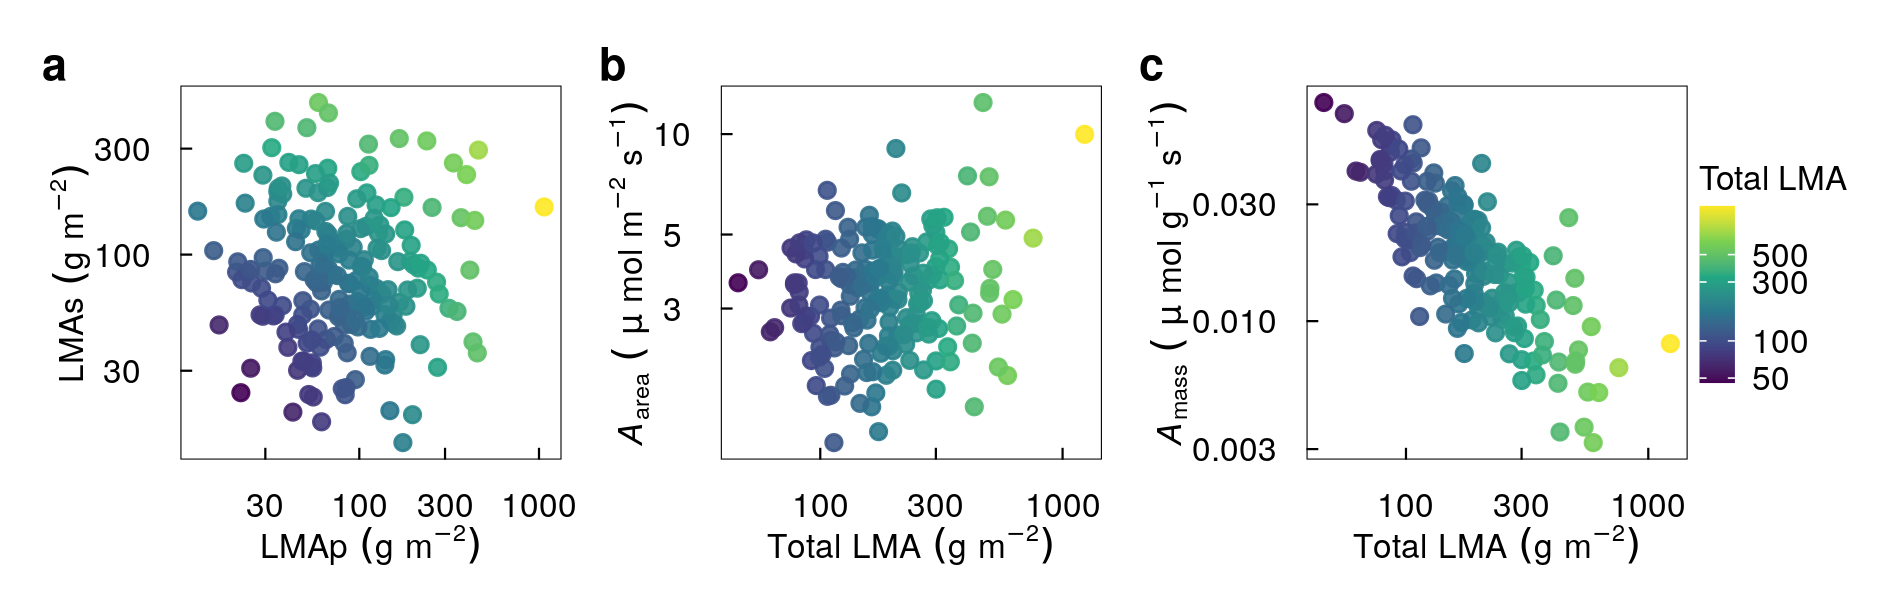
\includegraphics{../figs/hypo.png} \newpage

\textbf{Fig. 2:} 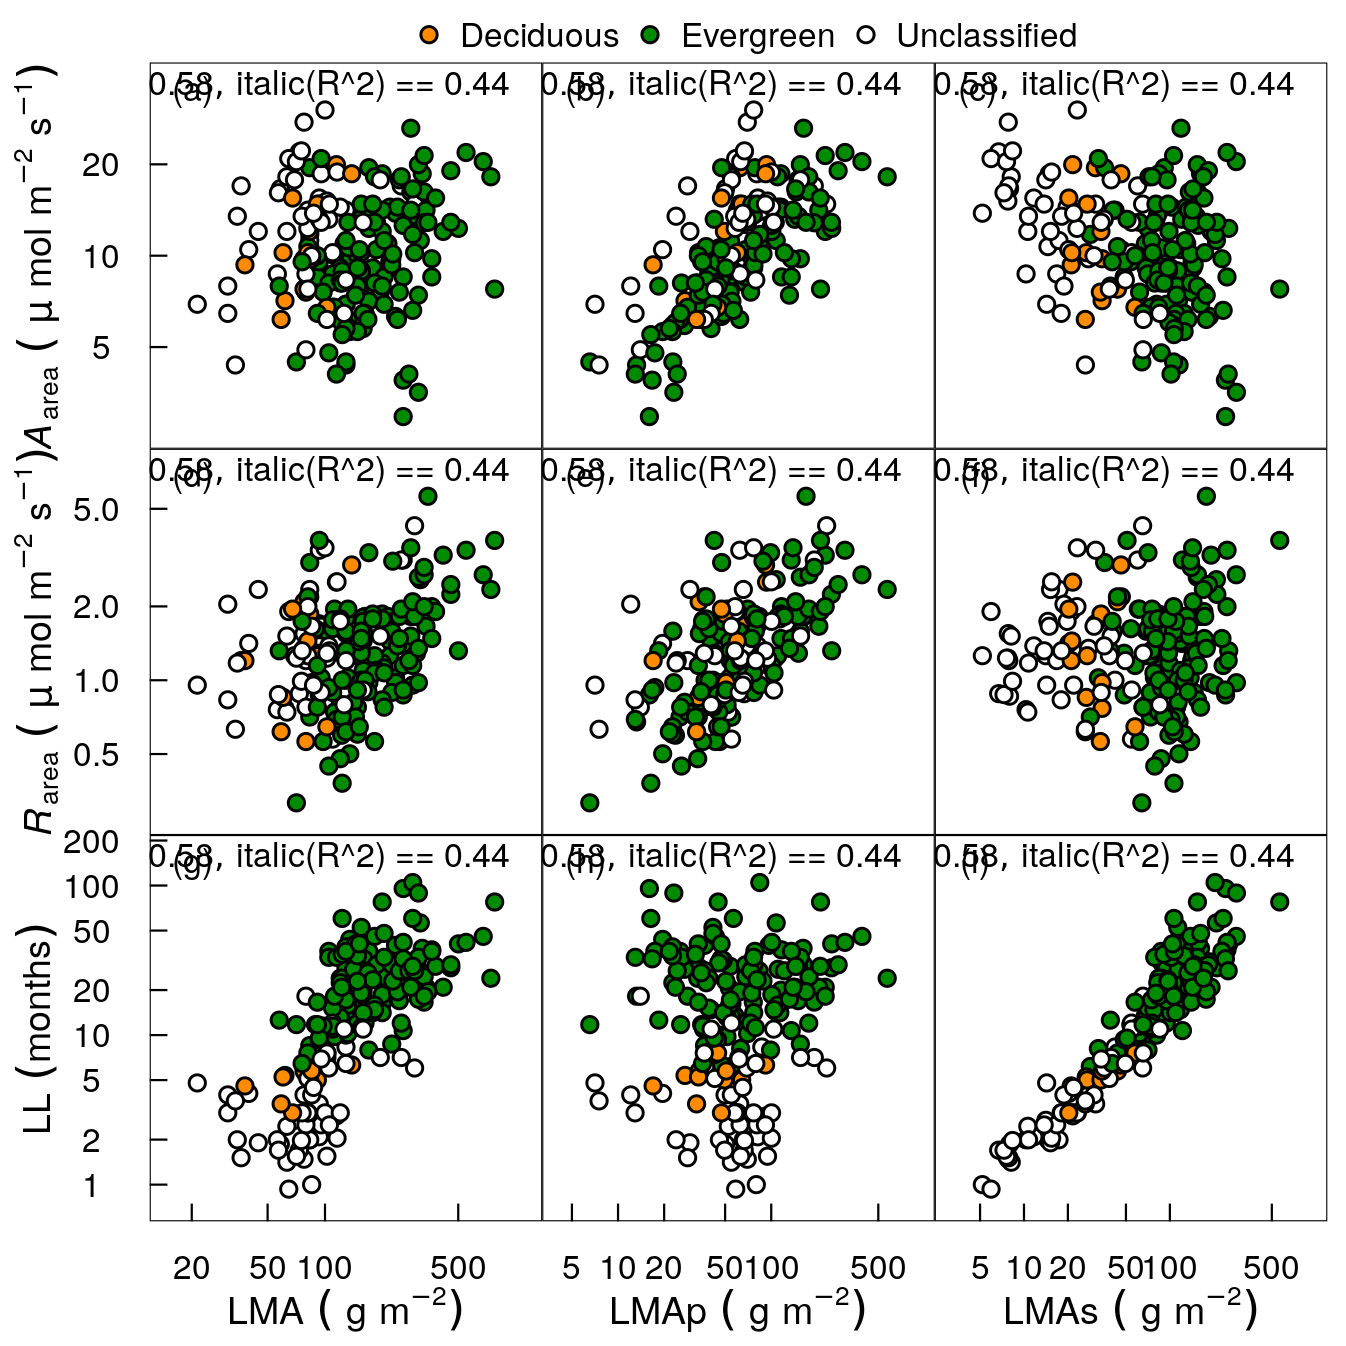
\includegraphics{../figs/gl_point.png} \newpage

\textbf{Fig. 3:} 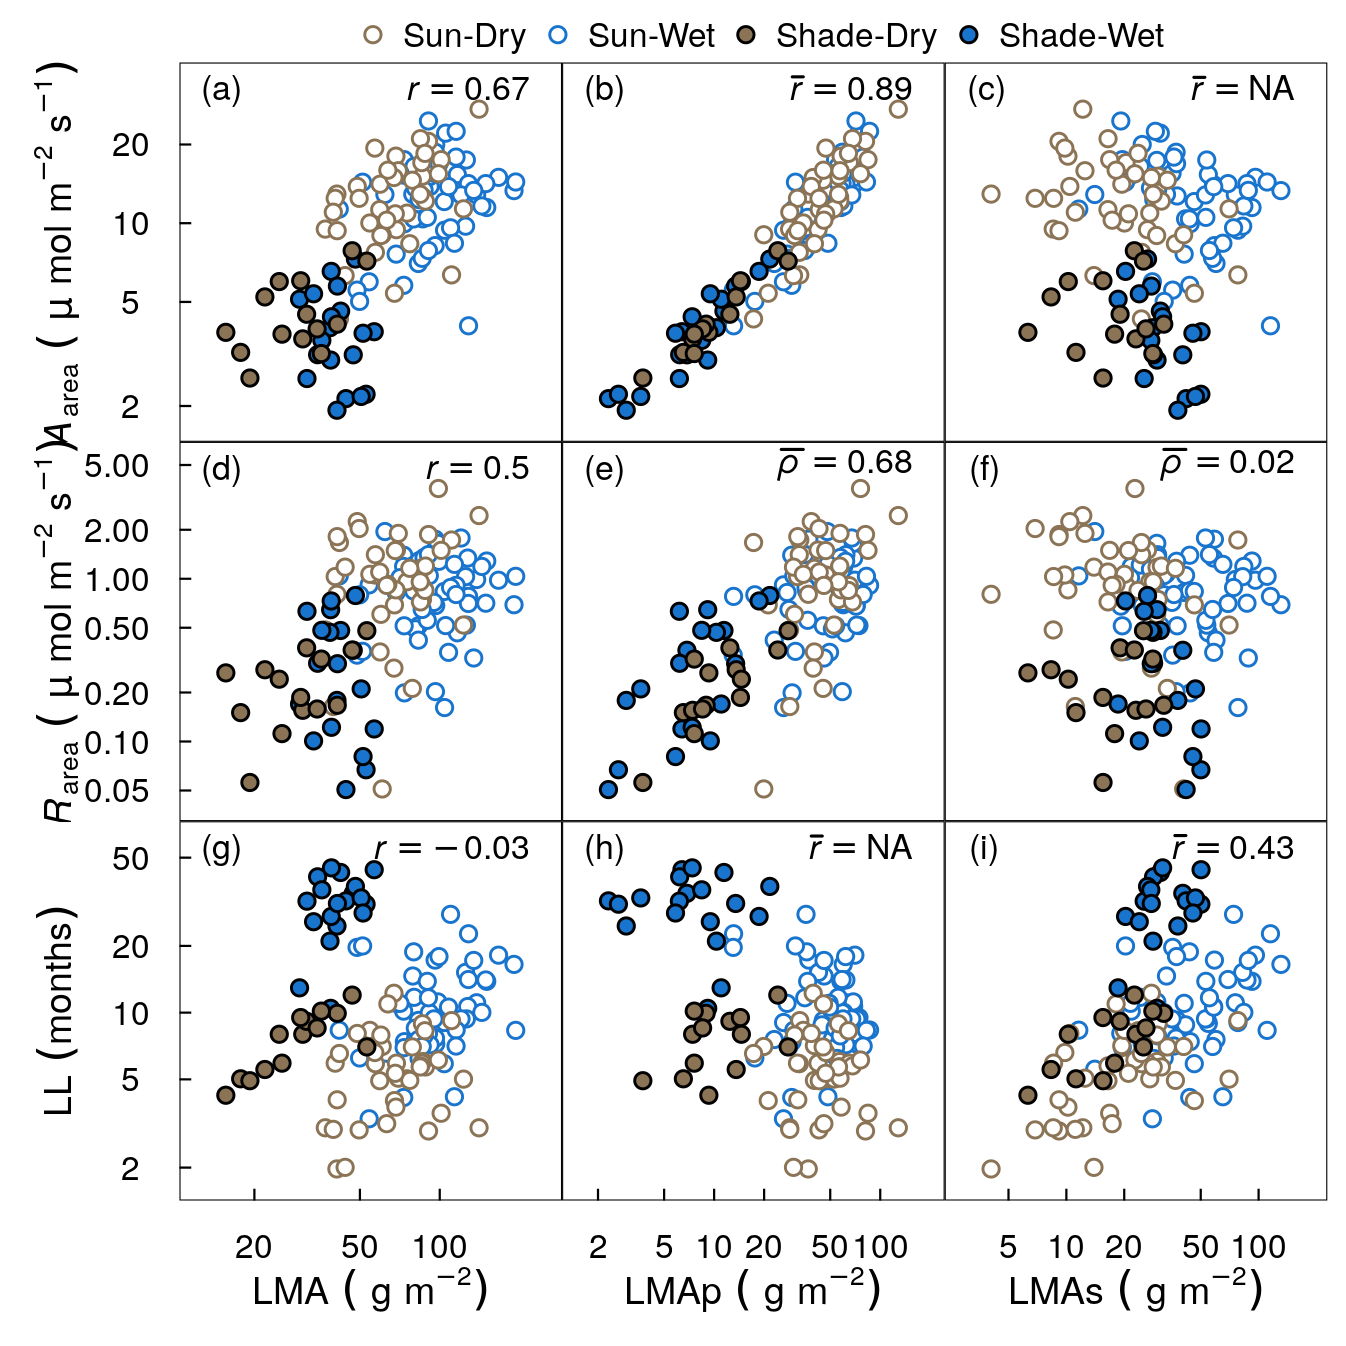
\includegraphics{../figs/pa_point.png} \newpage

\textbf{Fig. 4:} \includegraphics{../figs/pa_point_par_ll.png} \newpage

\textbf{Fig. 5:} \includegraphics{../figs/box_de.png} \newpage

\textbf{Fig. 6:} \includegraphics{../figs/box_pa.png} \newpage

\textbf{Fig. 7:} 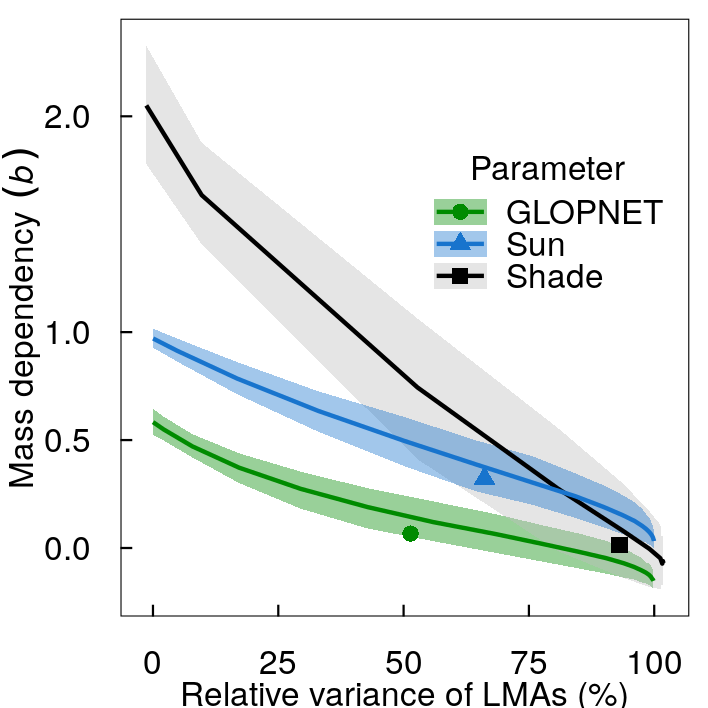
\includegraphics{../figs/mass_prop_mv.png}




\end{document}
